\documentclass{extarticle}
\usepackage{manualdoprofessor}
\usepackage{fichatecnica}
\usepackage{lipsum,media9,graficos}
\usepackage[justification=raggedright]{caption}
\usepackage{bncc}
\usepackage[kalinka]{../edlab}
\usepackage{marginnote}

\begin{document}


\newcommand{\AutorLivro}{Aleksei Tolstoi}
\newcommand{\TituloLivro}{Infância de Nikita}
\newcommand{\Tema}{Ficção, mistério e fantasia}
\newcommand{\Genero}{Romance}
\newcommand{\imagemCapa}{./images/PNLD0049-01.png}
\newcommand{\issnppub}{---}
\newcommand{\issnepub}{---}
% \newcommand{\fichacatalografica}{PNLD0049-00.png}
\newcommand{\colaborador}{\textbf{Marina Darmaros} é uma pessoa incrível e vai fazer um bom serviço.}


\title{\TituloLivro}
\author{\AutorLivro}
\def\authornotes{\colaborador}

\date{}
\maketitle

\begin{abstract}
\lipsum[1-3]
\end{abstract}

\tableofcontents

\pagebreak

\reversemarginpar
\marginparwidth=5cm

\section{Carta aos professores}

Caro educador / Cara educadora,\\\bigskip

O presente manual tem por objetivo oferecer apoio pedagógico àqueles
para quem o livro \emph{A infância de Nikita,} de Aleksei Tolstói
(1883-1945), foi pensado e preparado: educandos do ensino médio. A
pessoa fundamental para o sucesso desse encontro é justamente você, que
educa, a quem convidamos a mergulhar nas encantadoras memórias de
infância de um importante autor russo do século \textsc{xx}.

Trata"-se de uma tradução feita diretamente do russo para o português de
uma novela publicada inicialmente em 1922. Queremos apresentar a
literatura clássica russa juvenil por meio de um texto de fácil
compreensão e com um enredo que explora os dilemas e encantos da
meninice e da mocidade. Buscamos também ampliar o repertório de
clássicos da juventude com uma obra que dá ao leitor a oportunidade de
entrar em contato com uma cultura completamente diferente da dele,
alargando a percepção de si e do mundo.

O livro, de linguagem leve e cativante, traz questões literárias,
sociais e históricas que serão contextualizadas e aprofundadas nas
atividades aqui propostas, as quais incentivarão não só a pesquisa e a
produção de textos, mas também o desenvolvimento de outras
multimodalidades. O intuito deste manual é, no fim das contas, ajudar a
fazer da leitura um hábito e um prazer na vida de jovens do ensino
médio.

Esperamos que achem este material proveitoso para o trabalho em sala de
aula!


\section{Atividades 1}

\bnccativividadespreleitura
\BNCC{EM13LP07}
\BNCC{EM13LP46}
\BNCC{EM13LP49}
\BNCC{EM13CHS105}

Orientações para as aulas de Língua Portuguesa, preparando os
educandos para a leitura da obra (seção Pré"-leitura), assim como para
sua análise e problematização (Pós"-leitura).

\paragraph{Tema} Aprendendo sobre o gênero das memórias literárias.

\paragraph{Conteúdo}
Apresentação, leitura e compreensão de alguns trechos de \emph{A
infância de} Nikita e do gênero confessional de memórias literárias,
além do tratamento dado ao narrador e de alguns temas específicos
suscitados pelo livro. Trazemos algumas sugestões, mas o educador ou a
educadora podem fazer a curadoria dos trechos que considerarem mais
pertinentes à atividade.

\paragraph{Objetivos}
Ajudar o jovem leitor a se familiarizar com o gênero confessional das
memórias literárias, sobretudo as de infância, que nos levam a pensar a
escrita também como prática social, já que o educando acaba por conhecer
sua comunidade, o lugar em que ele vive e se insere. Diferenciar as
memórias literárias de outras escritas confessionais (diário e
autobiografia). Aprofundar a compreensão dos tipos de narrador e de
discurso. Refletir sobre certas peculiaridades da cultura russa e da
infância.

\paragraph{Justificativa}
As memórias de infância têm, em geral, grande apelo para o público jovem
devido à proximidade etária, à identificação com as aflições dos
personagens e ao prazer da leitura. Em \emph{A Infância de Nikita}, há
uma elaboração artística do teor autobiográfico: as fronteiras entre
realidade e ficção são propositadamente fluidas.

A questão do narrador surge com força e traz a oportunidade para o
estudo dos tipos de narrador (pré"-leitura) e de discursos (leitura).

Diferentemente de muitas memórias de infância em primeira pessoa (como
\emph{Infância, adolescência, juventude,} de Lev Tolstói,
\emph{Infância}, de Maksim Górki, ou a obra homônima de Graciliano
Ramos), o narrador destas memórias de Tolstói está em terceira pessoa,
mas usando com frequência o discurso indireto livre, ou seja,
expressando, por contágio e sem uma fronteira muito definida, a voz e os
sentimentos de Nikita, o protagonista.

Nikita, a quem o livro foi dedicado, era o nome do primogênito de
Aleksei Tolstói que, na época da escritura do texto, não passava de um
bebê, mas a história retrata os costumes e as lembranças da infância do
próprio autor --- a mãe da personagem Nikita tem, inclusive, o mesmo
nome da mãe de Tolstói, Aleksandra, e, apesar de o nome do pai diferir,
seu protótipo é claramente o do padrasto do escritor, Aleksei Bostrom
(em nome de quem Tolstói esteve registrado até os dezesseis anos), homem
bom, aventureiro, sonhador e um pouco atrapalhado nos negócios, como o
Vassíli Nikítievitch de Sosnovka.

Muitos escritores célebres registraram suas memórias de infância, que se
tornaram uma temática clássica do gênero confessional, que inclui
biografias, autobiografias, diários, etc. O gênero confessional, a
escrita de si, é talvez a forma de expressão que mais ganhou espaço nas
últimas décadas e, se pensarmos bem, é o gênero por excelência das redes
sociais que tanto ocupam a vida de jovens contemporâneos. Partindo de
formas de expressão conhecidas dos estudantes, é possível desenvolver
conceitos literários mais complexos.

Assim, a escrita confessional torna a obra de Tolstói uma excelente
porta de entrada para a literatura russa clássica, já que o autor, neste
livro, retoma a grande tradição literária russa do século \textsc{xix}.

\paragraph{Metodologia}
O educador pode iniciar em sala de aula uma leitura coletiva para
apresentar o texto e mostrar sua acessibilidade aos alunos. Essa leitura
pode ser feita a partir do primeiro capítulo do livro ou de trechos ou
capítulos escolhidos pelo educador. Seguem alguns pontos que podem ser
destacados durante esta atividade:

\subsection{Pré"-leitura}

Os episódios do livro não seguem uma sequência cronológica rigorosa e
um capítulo pode ou não estar ligado ao outro. Nesta obra, a sucessão de
tempo é percebida principalmente pela passagem demarcada das estações do
ano na Rússia e pelas festividades (Natal e Páscoa), como nota Mountian
(2021, Paratexto). Portanto, a memória literária não se quer precisa
como um diário, embora ela possa utilizá"-lo como base, e não tem a
pretensão de totalizar a existência, como na autobiografia. É a deixa
para que o educando coloque em discussão a escrita confessional.

As memórias e os diários guardam similaridades entre si, mas não são a
mesma coisa. Um dos diários mais famosos do mundo é o de Anne Frank, a
garota judia que, durante a Segunda Guerra Mundial, registrou seus dias
enquanto se escondia com sua família dos nazistas na parte de trás de um
apartamento de Amsterdã. Tome"-se um trecho do \emph{Diário de Anne
Frank} (1947):

\begin{quote}
Sábado, 20 de junho de 1942

Faz alguns dias que não escrevo porque eu quis, antes de tudo, pensar
neste diário. É estranho uma pessoa como eu manter um diário; não apenas
por falta de hábito, mas porque me parece que ninguém --- nem eu mesma
--- poderia interessar"-se pelos desabafos de uma garota de treze anos.
Mas que importa? Quero escrever e, mais do que isso, quero trazer à tona
tudo o que está enterrado bem fundo no meu coração.

{[}\ldots{}{]}

Vou explicar isso melhor, pois ninguém há de acreditar que uma menina de
treze anos se sinta sozinha no mundo. Aliás, nem é esse o caso. Tenho
meus pais, que são uns amores, e uma irmã de dezesseis anos. Conheço
mais de trinta pessoas a quem poderia chamar de amigas --- e tenho uma
porção de pretendentes doidos para me namorar e que, não o podendo
fazer, ficam me espiando, na classe, por meio de espelhinhos. Tenho
parentes, tios e tias, que também são uns amores, além de um lar
agradável. Aparentemente, nada me falta. (\textsc{frank}, 2003 p.27)
\end{quote}

Como comparação, tomemos agora um trecho das memórias de Maksim Górki,
intituladas \emph{Infância}:

\begin{quote}
Gravei na memória: a mãe não é forte; ela é como todo mundo, tem medo do
avô. Eu a impeço de ir embora da casa onde não consegue viver. Isso foi
muito triste. Em breve, de fato, a mãe sumiu de casa. Partiu para
hospedar"-se em algum lugar.

Um dia, de repente, como se tivesse caído do teto, o avô apareceu,
sentou"-se na cama, apalpou minha cabeça com a mão fria que nem gelo:

--- Bom dia, senhor\ldots{}. Vai, responda, não fique zangado!\ldots{} Bem, e
então?

Tive muita vontade de lhe dar um chute, mas mexer me causava dor. Ele me
pareceu ainda mais ruivo do que antes; sua cabeça balançava de um jeito
aflito; os olhos brilhantes procuravam alguma coisa na parede. Depois de
tirar do bolso um pão de mel em formato de bode, dois cartuchos de
açúcar, uma maçã e um cacho de passas azuis, colocou tudo no
travesseiro, perto do meu nariz.

--- Olhe aí, eu trouxe guloseimas para você.

(\textsc{górki}, 2010 p. 36-37)
\end{quote}

\marginnote{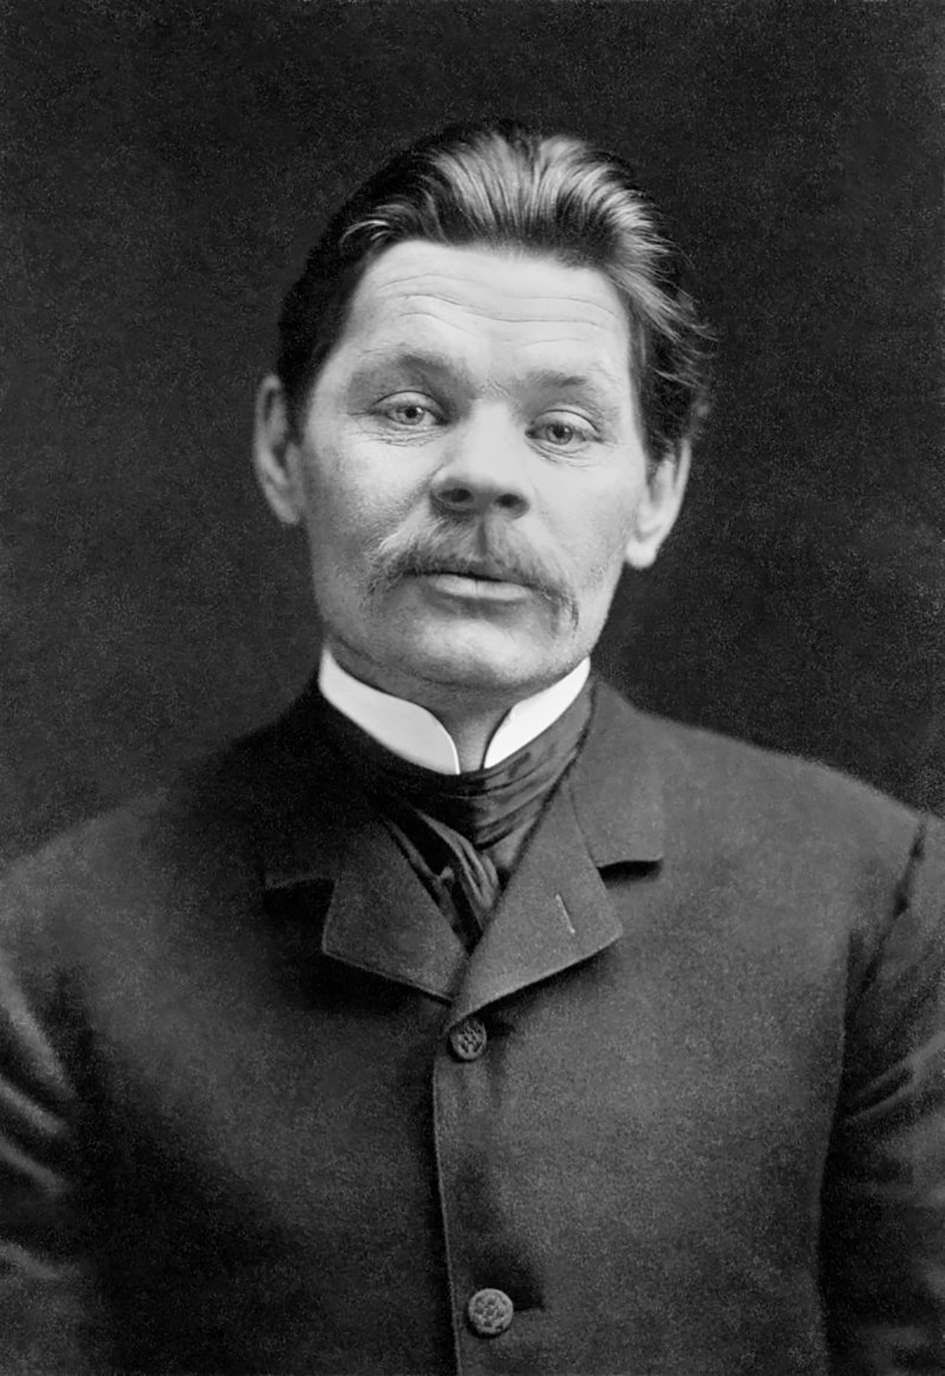
\includegraphics[width=5cm]{./images/PNLD0049-08.png}}

Como vemos, o diário, sempre narrado em primeira pessoa, concentra"-se no
tempo presente ou no passado recente, enquanto as memórias geralmente
tratam de acontecimentos de um passado mais distante, com um narrador em
primeira pessoa (como ocorre em Górki) e por vezes em terceira (como
veremos em Nikita).

O gênero das memórias literárias é um dos mais instigantes para o
trabalho em sala de aula, justamente por reinterpretar recordações com
mais liberdade, dando"-lhes tratamento literário e revelando lugares e
pessoas através de impressões próprias ou não, possibilidades que
distinguem as memórias da autobiografia, por exemplo. Mas estabelecer
limites claros entre os gêneros confessionais não é tarefa fácil.

\begin{quote}
Difícil traçar o limite exato entre a autobiografia, as memórias, o
diário íntimo e as confissões, visto conterem, cada qual a seu modo, o
mesmo extravasamento do ``eu''. Enquanto a autobiografia permite supor o
relato objetivo e completo de uma existência, tendo ela própria como
centro, as memórias implicam um à"-vontade na reestruturação dos
acontecimentos e a inclusão de pessoas com as quais o biógrafo teria
entrado em contato. Por outro lado, ao passo que o diário constitui o
registro dia a dia de uma vida, quer dos eventos, quer das suas marcas
na sensibilidade, as confissões decorrem do esforço de sublimar, pela
autorretratação, as vivências dignas de transmitir ao leitor. (\textsc{moisés},
2004, p. 46)
\end{quote}

A memória literária que faz uso do narrador em terceira pessoa, como é o
caso de \emph{A infância de Nikita,} está ainda mais à vontade,
parafraseando Moisés, na reinterpretação do passado: aqui as fronteiras
entre ficção e realidade não se querem delimitar, e a relação entre
autor e protagonista não é tão direta para o leitor como ocorre na
autobiografia.

Em \emph{Campo Geral} (1964), novela que compõe o livro \emph{Manuelzão
e Miguilim}, de Guimarães Rosa, o narrador que conta a história de
Miguilim, de oito anos, também muitas vezes se mistura ao protagonista
pelo discurso indireto livre. Aqui temos reminiscências de infância do
próprio Rosa em Cordisburgo e outras tomadas de empréstimo (inventadas
ou não). Aí reside outra característica que distingue as memórias da
autobiografia: nas primeiras não se espera necessariamente uma expressão
da realidade, do que ocorreu de fato, são baseadas em vivências, que
podem ser do autor ou de pessoas que ele conheceu, e envolvem apuro
estético; já a autobiografia, que muitas vezes não recebe tratamento
literário, busca estabelecer relação com a realidade mais factual (ou
com o que o sujeito apreende dela) e narrar uma história ampla de vida
(não raro o relato começa com o nascimento do autor"-narrador).

Para iniciar a atividade, sugerimos o primeiro capítulo de \emph{A
infância de Nikita}, que contêm informações interessantes para abrir a
leitura coletiva. Eles trazem o principal elemento que remete à Rússia
no imaginário brasileiro: a neve. Assim, antes de introduzir a leitura e
o debate sobre o gênero narrativo, o professor pode questionar os alunos
sobre o que lhes vem à mente quando se fala de Rússia (é a deixa para
lhes pedir que indiquem o país no mapa). Muitas imagens devem surgir:
frio, neve, ursos, vodca, talvez tenham visto alguns vídeos engraçados
na internet: qualquer lembrança é válida nesse momento. Pode"-se pedir
também algum tipo de atividade com este tema. Por exemplo: os educandos
fazem uma pesquisa, pela internet, na biblioteca ou entrevistas com
conhecidos, sobre o país, seus costumes e modos de diversão locais.

\subsection{Leitura}

\paragraph{Tema} Peculiaridades da cultura russa e da infância e
discursos do narrador.

Depois de discutida a escrita confessional, outras questões relativas ao
conteúdo e à forma poderão ser tratadas durante a leitura:

\begin{enumerate}
\item
Colorido russo

Conhecer uma nova cultura é o melhor exercício de alteridade, pois
amplia"-se a percepção de si e do outro. Os alunos certamente notarão a
presença de certos termos, como ``mujique'', ``isbá'' e ``samovar''
(todos explicados em notas de rodapé). São termos que, aliados aos
estranhos nomes e patronímicos dos personagens, introduzem o leitor no
universo russo.


Logo no primeiro capítulo, por exemplo, lidamos com um ``mujique'', o
camponês agregado a serviço do nobre ou o mais abastado. Esses
estrangeirismos não atrapalham o entendimento geral da obra nem
contaminam a tradução, mas trazem um colorido russo ao texto, abrem
questões que podem ser aprofundadas e ajudam a contextualizar a obra no
tempo"-espaço.

\marginnote{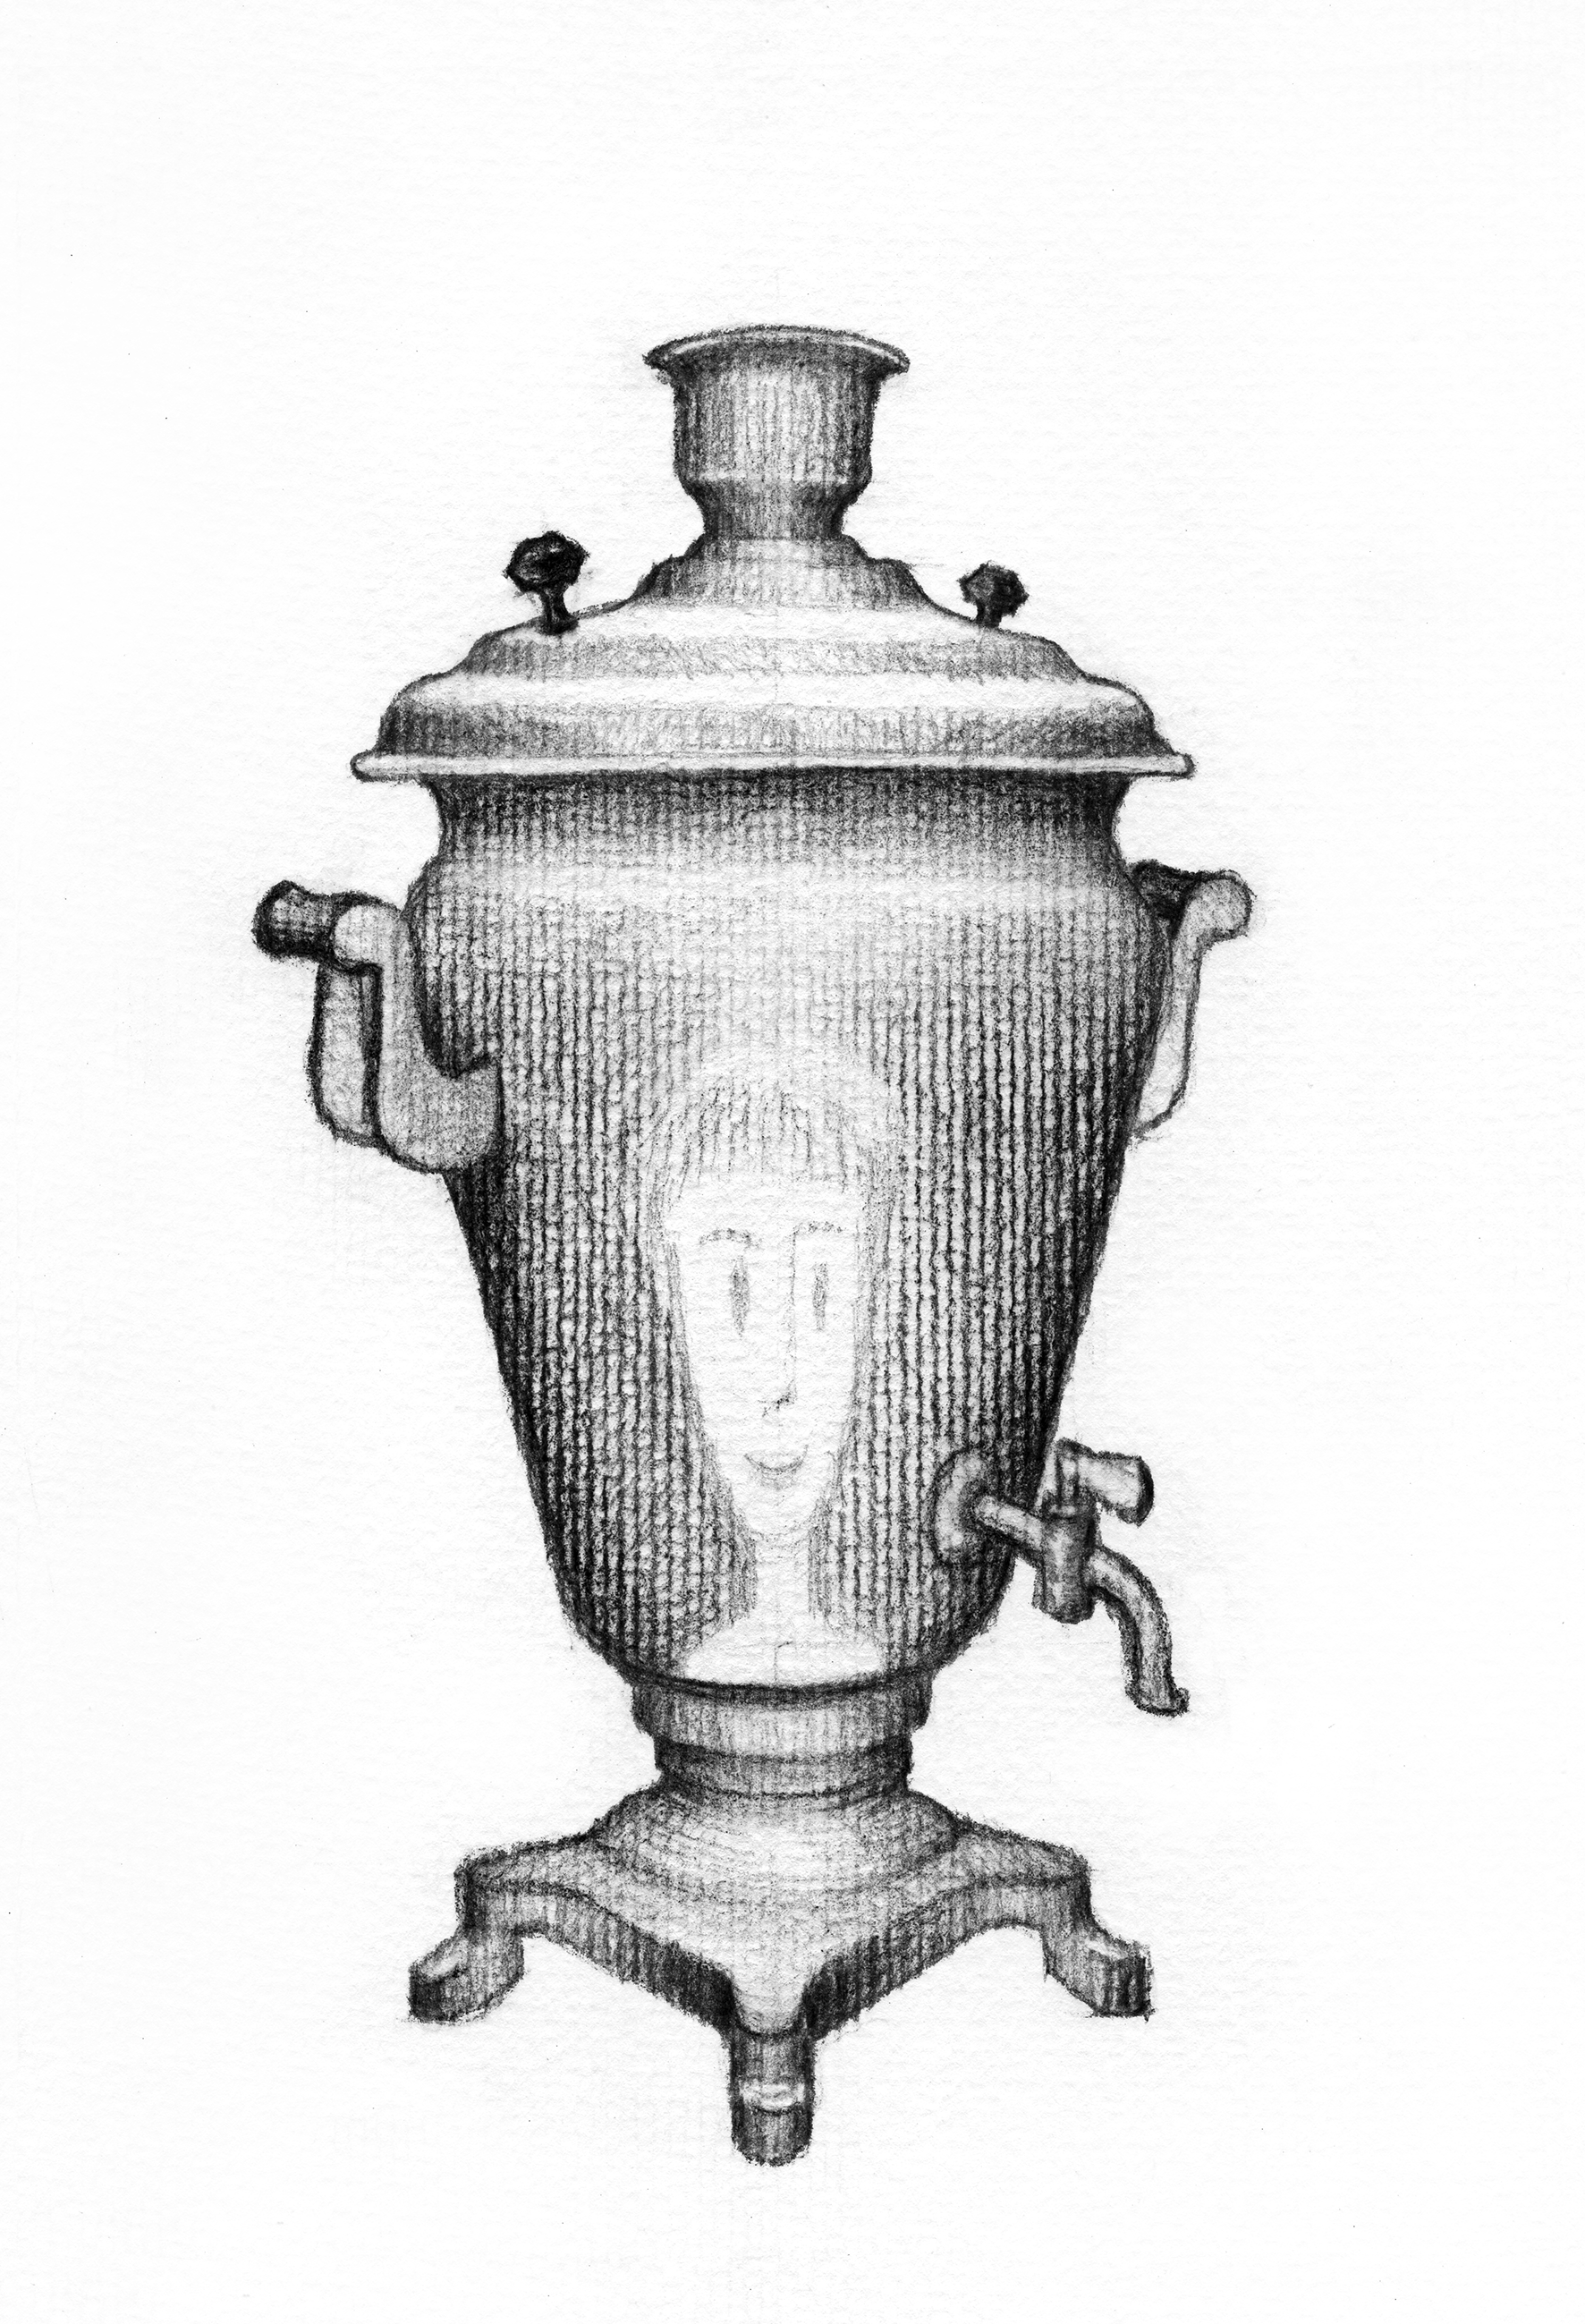
\includegraphics[width=5cm]{./images/PNLD0049-04.png}}

\item
Brincadeiras de infância

Quem não se lembra dos passatempos da meninice? Seja pega"-pega ou
\emph{game}? A história de Nikita permite refletir sobre as brincadeiras
de ontem e de hoje: o educando cria suas próprias memórias. Como
observou Mountian (2021, Paratexto), enquanto Lília, o primeiro amor de
Nikita, se ocupava com atividades caseiras (brincar de boneca, costurar,
etc.), os meninos brincavam ao ar livre e faziam seus próprios
brinquedos, como vemos nos primeiros capítulos. Posteriormente, surge o
tema da guerra, brincadeira clássica de meninos. No capítulo ``A
batalha'', há uma luta entre os garotos ``do nosso lado'' e os ``do
outro lado'', e Nikita dá uma surra no valentão Stiopka Karnaúchkin,
que, impressionado, convida"-o para ser seu amigo. Como são essas
relações na atualidade? Há diferenças? Meninos e meninas ainda se
dividem dessa maneira?

Outras questões sugeridas: Quais eram os meios de diversão dos russos
no século \textsc{xix} que aparecem no livro? Será que eles permanecem na
atualidade? As brincadeiras na neve, como o esqui, o trenó, teriam,
quiçá, equivalentes no Brasil (talvez no \emph{skate}, no surfe)? Quais
são os entretenimentos da infância e da adolescência hoje? Ocorrem
dentro ou fora de casa? São atividades coletivas ou individuais?
Envolvem trabalho manual?

\item
Hora de estudar

A leitura pode ser expandida também para a questão educacional com a
presença do preceptor Arkádi Ivánovitch. Os filhos de famílias nobres
começavam a ser educados em casa, daí a figura do preceptor (uma
realidade histórica do século \textsc{xix} que também ocorria no Brasil). Devido
à pandemia do coronavírus (2020/21), a discussão da educação em casa foi
transposta para os dias de hoje, com a transição do ensino presencial
para o virtual (meios \emph{on"-line}). Seria a volta da educação
domiciliar? Pode"-se traçar paralelos: se preceptores eram um privilégio
dos nobres e enriquecidos, a educação \emph{on"-line} é acessível a
todos? Todas as crianças têm acesso à internet, além de apoio familiar?
Também se pode pensar na relação que Nikita estabelecia com o estudo.
Ele gostava de estudar?

\item
Narrador e narrativa

Para aprofundar os procedimentos narrativos empregados por Aleksei
Tolstói, é possível lançar uma questão à classe: O narrador e o autor
são a mesma pessoa? O relato foi vivido pelo autor, mas é apresentado
por um narrador em terceira pessoa, em uma espécie de memória
``fantasmática'': ele dá ao protagonista o nome do filho, mas na
realidade é a própria vivência que retrata, misturando lembranças reais
e ficcionais e fazendo referências literárias:

\begin{quote}
Em obras em que o nome da personagem não coincide com o nome do autor na
capa, mas cuja história se assemelhe à do próprio autor, Lejeune afirma
haver um ``pacto fantasmático'', uma forma indireta de pacto
autobiográfico que convida o leitor a ler esses romances não apenas como
ficções, mas também como fantasmas que revelam um indivíduo.
(\textsc{velasco}, 2015, p. 3)
\end{quote}

Essa forma indireta de pacto é construída aqui principalmente pelo uso
do discurso indireto livre, em que as opiniões e os pensamentos da
personagem (em geral de Nikita) aparecem na voz do narrador. Esse tipo
de discurso é marca, aliás, da escrita de Clarice Lispector: todas as
suas obras utilizam dele. Em \emph{Nikita}, os exemplos são vastos:
``Nikita tinha a impressão de que, durante a multiplicação, o 1 e o 2
saltavam do papel para dentro de sua cabeça e lá faziam cócegas até que
fossem esquecidos\emph{. Isso era muito maçante}.'' (\textsc{tolstói}, 2021, p.
51, grifo nosso) Caso o trecho tivesse usado do discurso direto,
teríamos: ``Nikita disse: --- Isso é maçante''. Se do discurso indireto:
``Ele disse que aquilo era maçante.'' Os verbos dicendi (``falar'',
``dizer'', ``afirmar'', ``gritar''), que introduzem ou reproduzem
diálogos, são usados tanto no discurso direto como no indireto, enquanto
no discurso indireto livre não, por isso este requer do leitor mais
discernimento para identificar as diversas vozes do narrador.

Trechos em que a voz de Nikita e do narrador coincidem permeiam toda a
obra. Na p. 11: ``Arkádi Ivánovitch era um homem insuportável: sempre se
divertia, sempre piscava, não dizia nada diretamente, mas de um jeito
que afligia o coração'' --- aqui o narrador está quase na primeira
pessoa ao revelar os pensamentos de Nikita. Ou entre as páginas 20 e 21
(grifo nosso): ``O cavaleiro sem cabeça corria pelas pradarias,
chicoteando o capim alto; a lua vermelha se erguia sobre o lago. Nikita
sentia os pelos de sua nuca arrepiarem. Virou"-se cuidadosamente, e do
outro lado das janelas escuras passou uma sombra cinzenta.
\emph{Palavra, ele a viu}.'' Ou, ainda, na pág. 23 (grifo nosso): ``A
caixa não tem proteção de vidro. A qualquer momento sua pata alcançará o
pêndulo. \emph{Ah, se pudesse gritar\ldots{}''.}

Por fim, vale pensar na verossimilhança do texto. Será que é
verossímil? É descritivo? O educando pode aqui citar exemplos de trechos
mais verossímeis ou menos, mais descritivos ou menos. Em geral, cenas ao
ar livre, na natureza, são retratadas com realismo e vivacidade, estilo
que marcou Tolstói, conhecido como um mestre da descrição. Já as ações
que ocorrem dentro de casa usam de elementos fantásticos, não realistas.
\end{enumerate}

\paragraph{Tempo estimado} Três a quatro aulas de 50 minutos.

\subsection{Pós"-leitura \textsc{i}}

\bnccativividadesposleitura

\BNCC{EM13LP14}
\BNCC{EM13LP15}
\BNCC{EM13LP18}
\BNCC{EM13LP46}
\BNCC{EM13LP53}

Espera"-se que os educandos assimilem as questões básicas que envolvem
a memória literária. Os elementos indicadores do discurso indireto livre
também podem ser ressaltados: tempo verbal (imperfeito ou futuro do
pretérito, pretérito"-mais"-que"-perfeito) e uso de advérbios (jamais, ali,
lá, naquele momento), ausência de indicação de diálogo e de verbo
dicendi e permanência de interrogações e exclamações da forma oracional
originária. O educador pode também aprofundar alguma ideia discutida no
texto, realizar atividades escritas e orais ou avaliações, com o
objetivo de aferir o desempenho dos alunos em relação à leitura e
compreensão da novela. No trabalho com memórias, é importante que os
educandos assimilem a maneira como o escritor observou o evento
cotidiano e deu a ele uma forma literária.

\paragraph{Tema} Laboratório de escritores \emph{Instagrammers}: trabalhando a escrita de memórias.

\paragraph{Conteúdo} Criação de textos e divulgação da prática literária.
O ideal é que cada aluno escreva em primeira pessoa sobre suas próprias
experiências (pode ser de um evento, de uma viagem, de um encontro, de
umas férias, etc.); o texto, de uma folha, deve ser ilustrado com uma
imagem, que poderá depois ser publicada no \emph{Instagram} ou outra
rede social acompanhada da escrita (no estilo que se convencionou chamar
nas redes de ``textão''). Também haverá a possibilidade de escolher dar
voz a avô, avó, outro parente ou conhecido --- o estudante deve
entrevistar o protagonista e redigir breves memórias sobre algum
acontecimento ligado a ele, em primeira pessoa (ele falará do ponto de
vista do personagem) ou em terceira, de preferência com uso do discurso
indireto livre. A ideia é que o jovem transforme a experiência própria
ou alheia, colhida por meio de entrevista, em memórias literárias com
base nos conceitos adquiridos nas atividades anteriores. Podem ser
organizados grupos ou rodas de discussões dos temas/objetos a serem
tratados, mas a redação das memórias deverá ser individual.

\paragraph{Objetivos}

Tem como objetivo central incutir nos alunos o hábito de ler e escrever,
incentivando a produção de gêneros confessionais e incluindo
efetivamente a prática da escrita na rotina escolar. O estudante será
motivado a entrar no universo literário por meio de uma ferramenta (as
redes sociais) que lhe é muito próxima e familiar. Ao final do
laboratório, os educandos deverão ser capazes de:

\begin{enumerate}
\item
Organizar e estruturar textos literários;

\item
Compreender o conceito de textualidade tendo como base a coerência e a
coesão;

\item
Produzir textos com linearidade e fluidez ou propositadamente
desconstruídos, já que também é possível organizar as memórias de forma
não linear e não cronológica, com o uso de \emph{flashbacks} ou de
outros procedimentos;

\item
Estruturar narrativas subjetivas e objetivas, diferenciando"-as e
utilizando"-as em determinadas situações;

\item
Utilizar recursos e variação linguística de acordo com o contexto
situacional e as características da personagem.
\end{enumerate}

\paragraph{Justificativa}
O Laboratório de Escritores \emph{Instagrammers} visa à preparação dos
alunos do ensino médio para desenvolvimento da leitura e escrita de
textos, tanto para a realização de avaliações externas como para
incrementar o ensino da leitura e da escrita na escola. Visa"-se,
portanto, à preparação de competências e habilidades para a construção
de um texto com qualidades literárias, com exploração expressiva de
variedades linguísticas, recursos de linguagem (como metáforas,
comparações) e progressão narrativa, assim como para o entendimento de
propostas de redação e de atividades simples de leitura e escrita, e ao
estímulo à leitura de autores diversos que tenham praticado o gênero das
memórias. A ideia é que o laboratório constitua agrupamentos de
estudantes para observação, discussão e produção nessa área de estudo,
desenvolvendo, além dos objetivos específicos referidos acima, autonomia
e iniciativa dos educandos.

\paragraph{Metodologia}
A primeira parte do projeto consiste na formação de grupos de estudantes
e de professores, que poderão acompanhar o laboratório e guiá"-lo, além
da definição da periodicidade dos encontros. As reuniões do laboratório
poderão ser realizadas na biblioteca da escola, assim como no auditório,
no teatro ou em alguma sala escolhida para tal fim, e reunir alunos de
diferentes turmas do ensino médio.

As atividades iniciais poderão consistir em uma discussão da obra, tendo
como base as questões propostas neste manual. Em seguida, os escritores
do laboratório poderão ampliar o repertório do grupo, discutindo e
listando outras sugestões de leitura do gênero e levantando questões
sobre a importância das memórias de infância/adolescência
especificamente. É aqui também que os alunos definirão se relatarão
experiências próprias ou de outras pessoas --- compartilhando com os
colegas, neste caso, o personagem que incorporará ao texto e que será,
em fase seguinte, entrevistado. Caso o protagonista seja o próprio
autor, ele falará à turma sobre a seleção das memórias que entrarão no
texto. Pode"-se inserir na atividade, também, a questão da variação
linguística, dos diversos usos que se pode fazer da linguagem em
contextos e plataformas diversas. As redações poderão ser reunidas em um
tomo \emph{on"-line} posteriormente e apresentadas nas reuniões ou em
evento aberto. Além disso, poderão ser publicadas pelos alunos em redes
sociais próprias ou coletivas (é possível se criar uma página no
Facebook, por exemplo, para a difusão dos trabalhos).

\paragraph{Tempo estimado} Seis a oito reuniões de 50 minutos.

\subsection{Pós"-leitura \textsc{ii}}

\paragraph{Tema} A construção da personagem e estéticas literárias em \emph{A infância de Nikita}.

\bnccativividadesposleitura
\BNCC{EM13LP52}

\paragraph{Conteúdo}
Análise de texto aplicando a base teórica estudada nas aulas de
literatura. Através do desenvolvimento linguístico e cultural trabalhado
nas aulas, o estudante poderá aprimorar capacidades importantes: a
leitura, a escrita e a interpretação de elementos relevantes, além de
criar novas conexões entre teoria e prática literária e o contexto
sócio"-histórico.

\paragraph{Objetivos}
A atividade incentiva os educandos a ler, escrever e interagir com o
texto, desenvolvendo também seu senso crítico e sua inserção no processo
de letramento social. Além disso, eles poderão aplicar os conhecimentos
teóricos estudados nas aulas de literatura.

\paragraph{Justificativa}
Considerada por alguns críticos a melhor obra de Aleksei Tolstói,
\emph{A infância de Nikita} descreve um ano da vida de um menino entre
os nove e os dez anos de idade, quando ele morava numa propriedade em
Sosnovka ao lado da mãe, do pai e do preceptor, no fim do século \textsc{xix}. De
um inverno a outro, o narrador introduz episódios significativos para a
personagem principal (e para o autor). Não por acaso, o livro trata do
início da puberdade, assimilando alguns elementos do romance de formação
ao mostrar certo amadurecimento de Nikita após enfrentar os desafios e
as mudanças do fim da infância.

A novela se inicia literalmente com o despertar de Nikita (``Nikita deu
um suspiro ao despertar e abriu os olhos''); permeada de elementos
românticos e simbólicos, é constituída por capítulos curtos. São cenas
fugazes do cotidiano de uma infância em meio à natureza.

Além do caráter confessional, o autor estabelece um diálogo intertextual
com a obra de sua mãe, a escritora Aleksandra Bostrom (1854-1906), e a
de outros autores, como Aleksandr Púchkin, Maksim Górki e Lev Tolstói,
remontando à tradição literária russa do século \textsc{xix}. (\textsc{mountian}, 2021)

\paragraph{Metodologia}
Diversos trechos da obra podem ser analisados separadamente, ressaltando
seus elementos românticos e outros recursos narrativos utilizados pelo
autor. Alguns pontos podem ser levantados:

\begin{enumerate}
\item
A estética romântica e elementos fantásticos

A certa altura da novela o menino se vê apaixonado por Lília, filha de
Anna Apolóssovna, amiga da mãe que tinha vindo de Samara para as festas
natalinas. Surge o tema do primeiro amor:

\begin{quote}
--- Como está vermelho --- disse Lília ---, parece uma beterraba.

E de novo se inclinou sobre a caixinha. Seu rosto tornou"-se astuto.
Nikita parecia grudado à cadeira. Não sabia o que dizer e não conseguia
sair do quarto de modo algum. A menina ria dele, mas ele não ficou
magoado nem zangado, e somente a admirava. (\textsc{tolstói}, 2021, p. 60)
\end{quote}

O amor de Nikita é descrito com ``notas gótico"-românticas''. Um
exemplo está no sonho cheio de mistério (elemento recorrente no
romantismo) de Nikita, com um gato debaixo do sofá, um relógio de
parede, quadros ganhando vida, reflexos da lua sobre o piso da velha
casa\ldots{} Realidade e sonho se fundem quando o menino conta a Lília o
sonho que tivera com o escritório de seu estranho bisavô, que tanto
havia sofrido pela mulher amada (o amor romântico que não se realiza).
Ao ouvir o relato de Nikita, Lília pergunta o que havia no vaso sobre o
relógio que tinha aparecido no sonho e, sem resposta, ambos vão até o
escritório, iluminado pela lua, e no vaso encontram um anel. Criando um
efeito cinematográfico, o gato da casa sai correndo nesse instante.

Elementos fantásticos e simbólicos surgem aqui e ali na obra de
Tolstói. Não por acaso alguns críticos chamaram seu estilo de ``realista
simbólico'' O vento uivando no sótão, o corvo que parecia o diabo, o
gato de olhos dissimulados\ldots{}

\marginnote{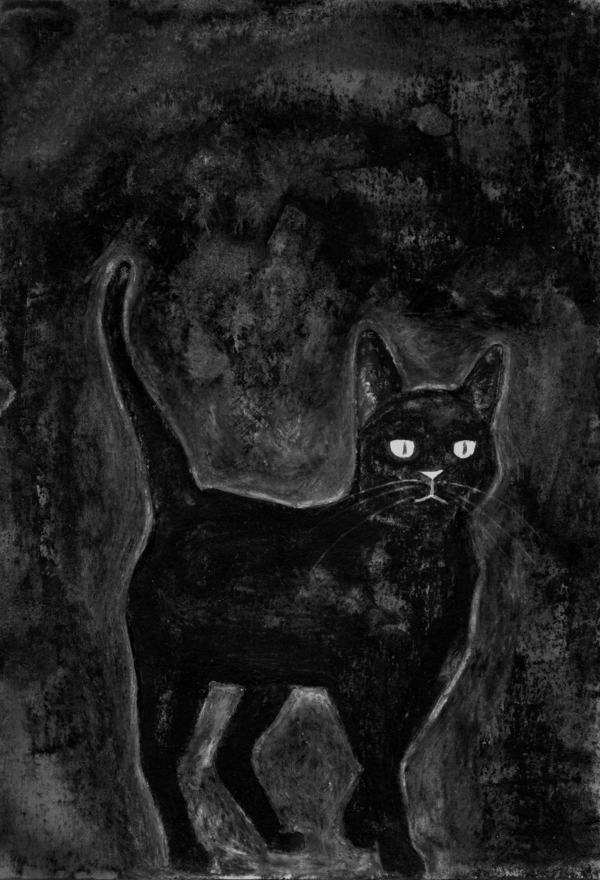
\includegraphics[width=5cm]{./images/PNLD0049-09.png}}

\item
Animais e natureza

Nikita estava rodeado de animais de estimação, o gato Vassíli, o
ouriço Akhilka, o cavalo Klópik, mas decerto os laços mais fortes ele
criou com o estorninho de que começou a cuidar, depois de ter completado
dez anos. O estorninho Jeltúkhin, que falava e pensava, foi conquistado
por Nikita; após ter sido salvo das garras do gato pelo menino, chegou à
seguinte conclusão: ``Não há no mundo animal mais forte do que Nikita''
(\textsc{tolstói}, 2021, p. 154). A partir desse dia, o pássaro se deixou
acariciar, pulava no ombro de Nikita, que construiu uma casa para ele. O
passarinho ficou ali até agosto, quando partiu, juntamente com as aves
migratórias, mas voltou, trazendo sinais: foi quem anunciou que choveria
quando a família, preocupada com a lavoura, enfrentava a seca.

O estorninho tornou a partir, deixou"-se ir, assim como Nikita deixou"-se
levar pelos afazeres, sem responder uma carta de amor que recebera de
Lília.

A partida do pássaro foi a segunda experiência de perda vivenciada por
Nikita, mas dessa vez o menino não pareceu se importar, como observa
Mountian (2021, Paratexto). A narrativa estabelece estreita ligação
entre o menino e o pássaro. Depois de Nikita, a personagem com quem o
narrador mais se confunde é com o estorninho: ele assume a perspectiva
do pássaro algumas vezes, aproximando"-se e afastando"-se da personagem,
quase como uma câmera. No fim do livro, após a mudança da família para
Samara, lemos: ``Mas Nikita, como seu estorninho atrás da tela de gaze,
sentia"-se um prisioneiro que fora apanhado, um alheio, era como
Jeltúkhin, sem tirar nem pôr''. (\textsc{tolstói}, 2021, p. 203)

``O campo, idealizado na propriedade de Sosnovka, é um depositório de
experiências de iniciação, mediadas por animais, por fenômenos da
natureza e pelas estações do ano'' (\textsc{mountian}, 2021, Paratexto) A
efemeridade e a transitoriedade da infância são sinalizadas pelas
transformações da natureza. As estações do ano são muito mais demarcadas
na Rússia do que no Brasil e não raro temperam os sentimentos das
personagens. O inverno para Nikita era sinônimo de despertar, de
brincadeiras na neve, de férias de Natal (os meses de inverno russo vão
de dezembro a março). O fim do inverno, pouco antes do degelo, traz
angústia a Nikita e isso coincide com a partida de Lília. As enchentes
do degelo trazem de volta o pai de Nikita, Vassíli Nikítievitch, que
quase morreu afogado com Lord Byron, seu garanhão (a primeira tempestade
simbólica do livro). A estadia do pai é um misto de ânimo e confusão,
começam as atividades primaveris antes da semeadura. Também na
primavera, quando tudo ao redor começa a florescer, Nikita completa 10
anos, em 11 de maio. Partidas são sempre nostálgicas, dando o tom do fim
da obra: Nikita parte para sua vida na cidade ``num dia outonal,
cinzento e ventoso''. (\textsc{mountian}, 2021, Paratexto)

\marginnote{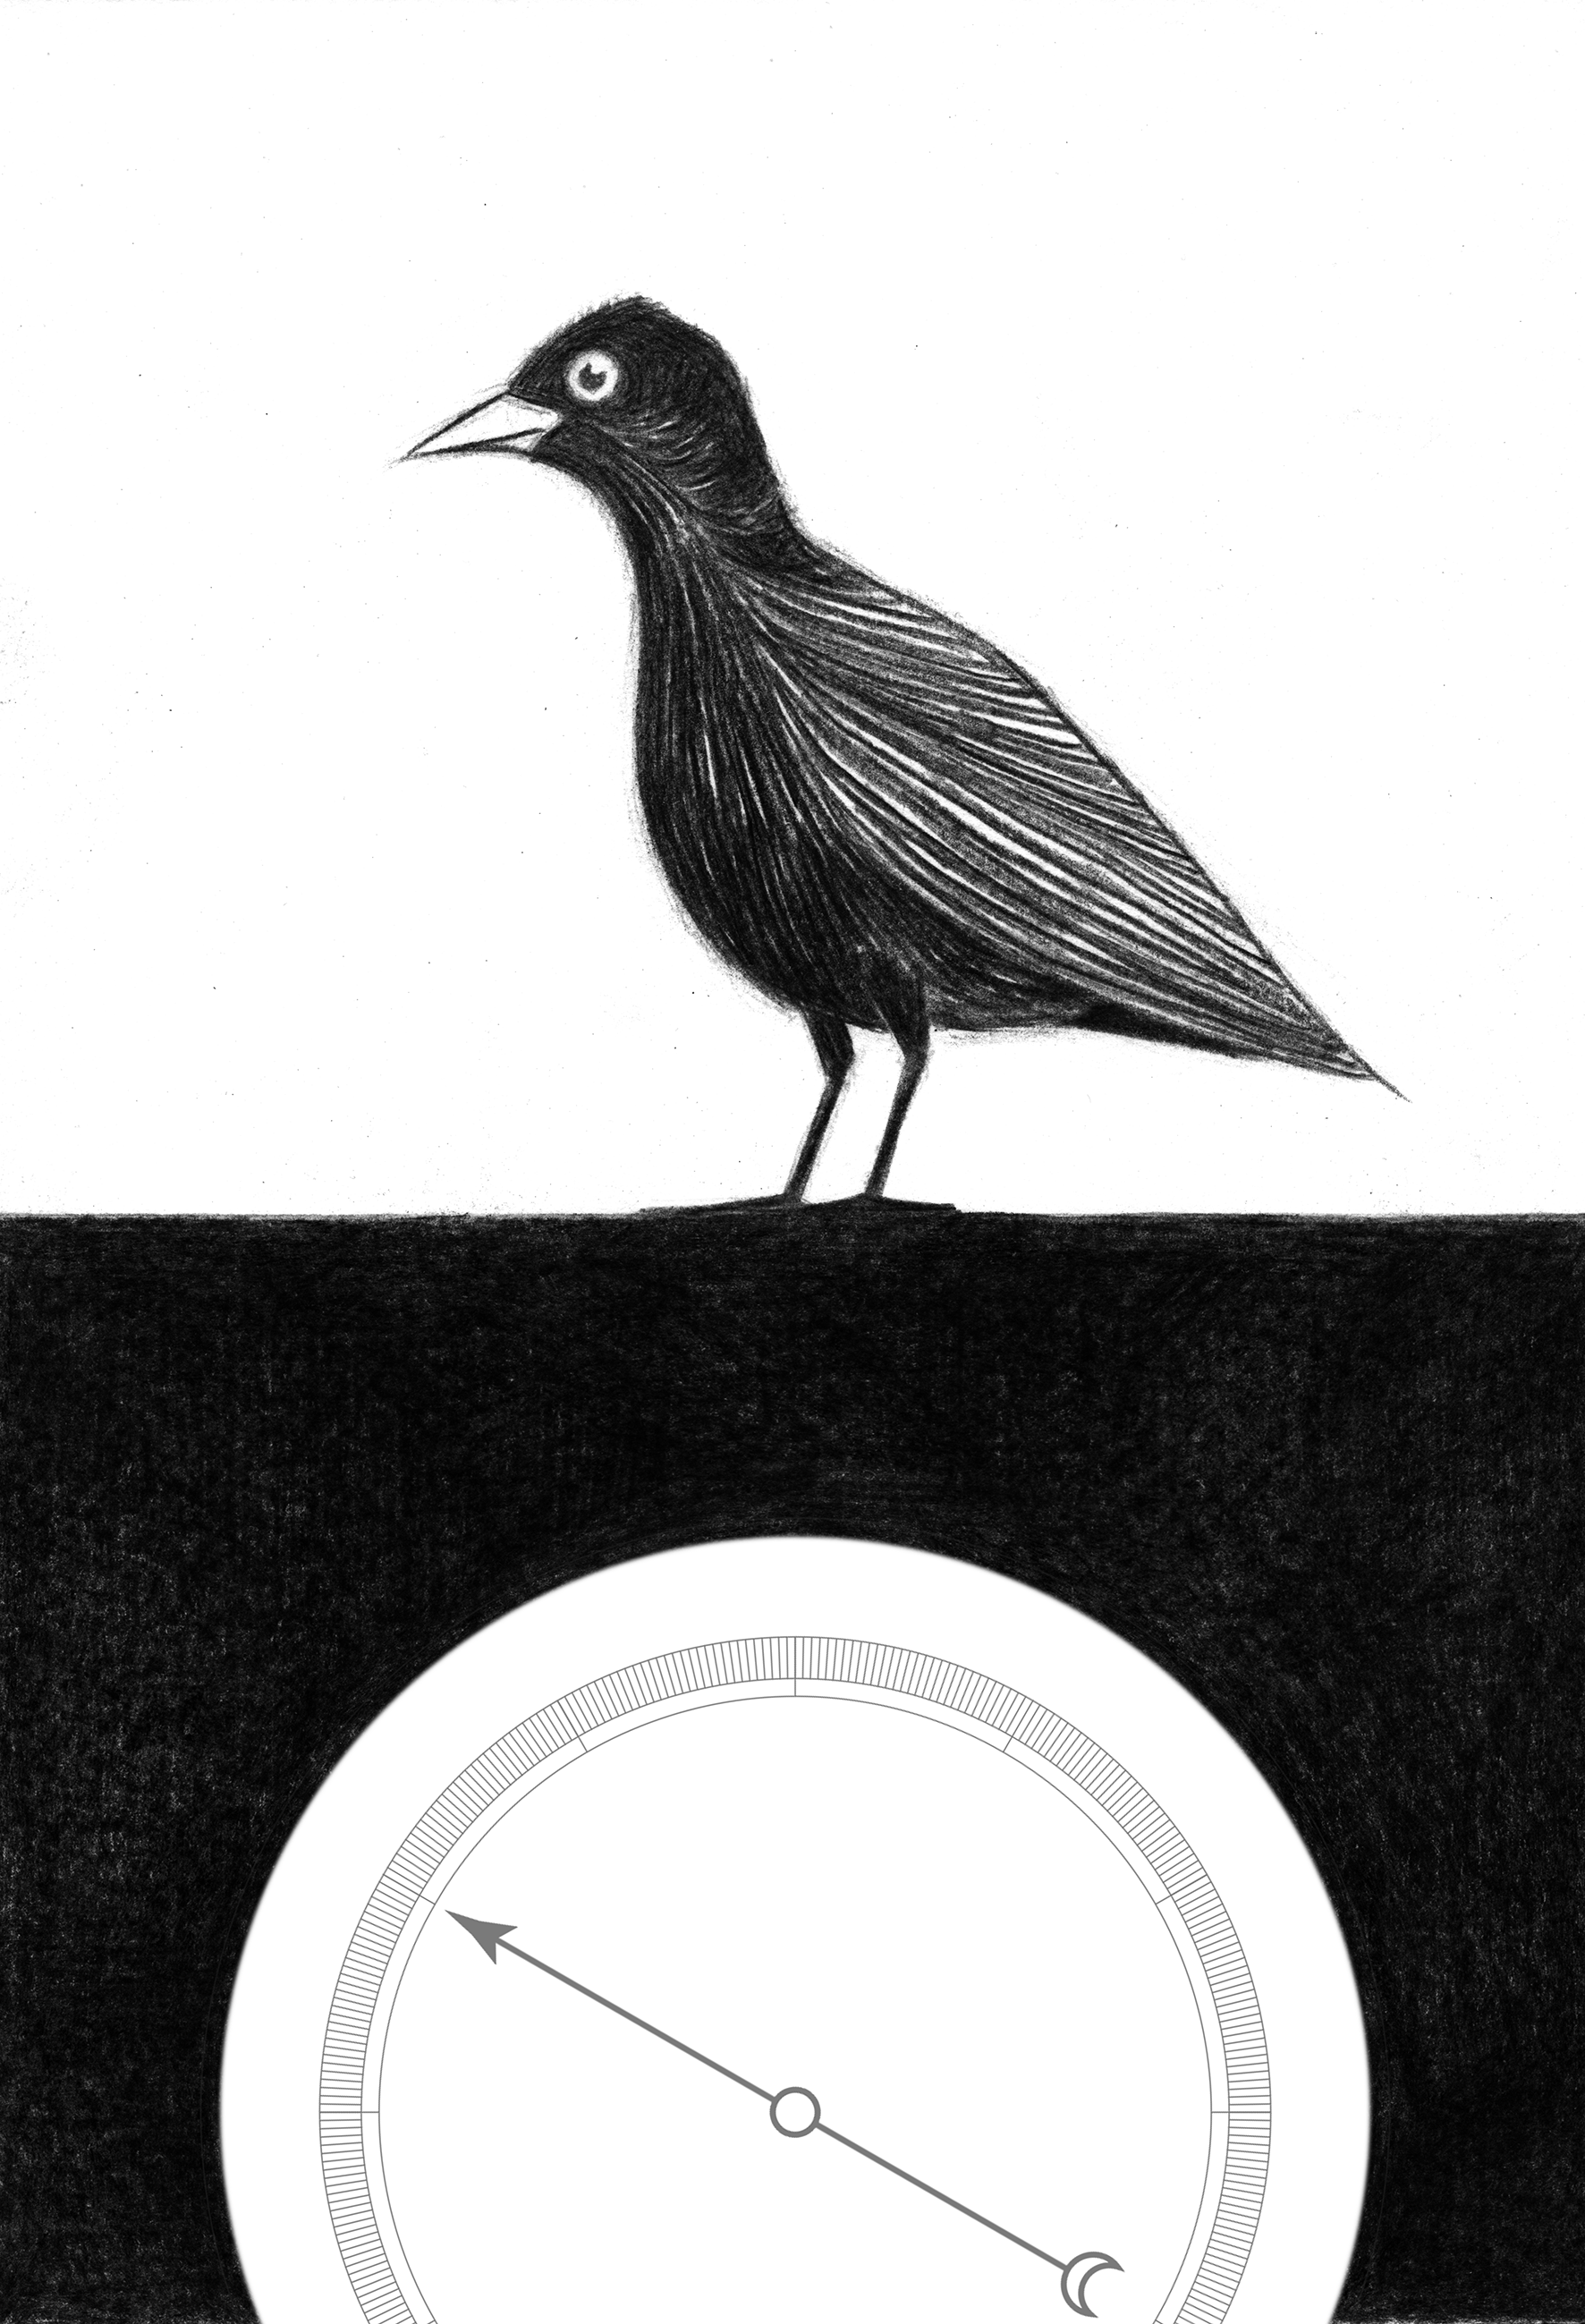
\includegraphics[width=5cm]{./images/PNLD0049-05.png}}

A natureza também surge como representação da Rússia. O campo funciona
como ligação ao país --- a natureza como refúgio de nacionalismo (mais
um elemento romântico). É preciso lembrar que, durante a criação desta
obra, Tolstói encontrava"-se no estrangeiro, enquanto seu país natal
passava por uma guerra civil.

A natureza também marca os primeiros e ingênuos versinhos que Nikita
escreveu e deu a Lília:

\begin{verse}
Ah, tu, bosque, meu bosque,\\
Meu encantado bosque,\\
Cheio de aves e animais\\
E feras joviais\ldots{}\\
Eu te amo, meu bosque\ldots{}\\
Como eu te amo, bosque\ldots{}
\end{verse}

A oposição campo \emph{versus} cidade é assinalada algumas vezes ao
longo do livro, mas no fim isso se acentua: fica claro que a infância de
Nikita termina justamente quando ele se muda para Samara. A vida na
cidade grande, que para ele era suja e sufocante, demarcou um
amadurecimento na personagem: ele se despediu da infância e de sua amada
Sosnovka.

\item
A construção da personagem

Nikita não era um menino de temperamento ruim, mas estava longe de ser
exemplar: não gostava, por exemplo, de seu preceptor: ``Um sujeito
surpreendentemente desenvolto e esperto era esse Arkádi Ivánovitch''.
(\textsc{tolstói}, 2021, p. 10) O tédio com que Nikita tem as lições de
aritmética é contornado pela imaginação fértil:

\begin{quote}
``Um lojista vendeu alguns \emph{archins} {[}medida russa equivalente a
0,71 m.{]} de tecido azul a 3 rublos e 64 copeques o \emph{archin}, e de
tecido preto a\ldots{}'' --- leu Nikita. Imediatamente, como costumava
acontecer, aquele lojista do livro de exercícios surgiu"-lhe na
imaginação. Estava de sobrecasaca comprida e empoeirada, o rosto amarelo
e desanimado, uma figura enfadonha, achatada e magra. Sua lojinha era
escura, como uma fenda; numa prateleira empoeirada se achavam duas peças
de tecido; o lojista esticava as mãos magras, tirava as peças da
prateleira e fitava Nikita com olhos opacos e sem vida.
(\textsc{tolstói}, 2021, p. 12-13)
\end{quote}
\end{enumerate}

\paragraph{Tempo estimado} Duas a três aulas de 50 minutos cada.


\marginnote{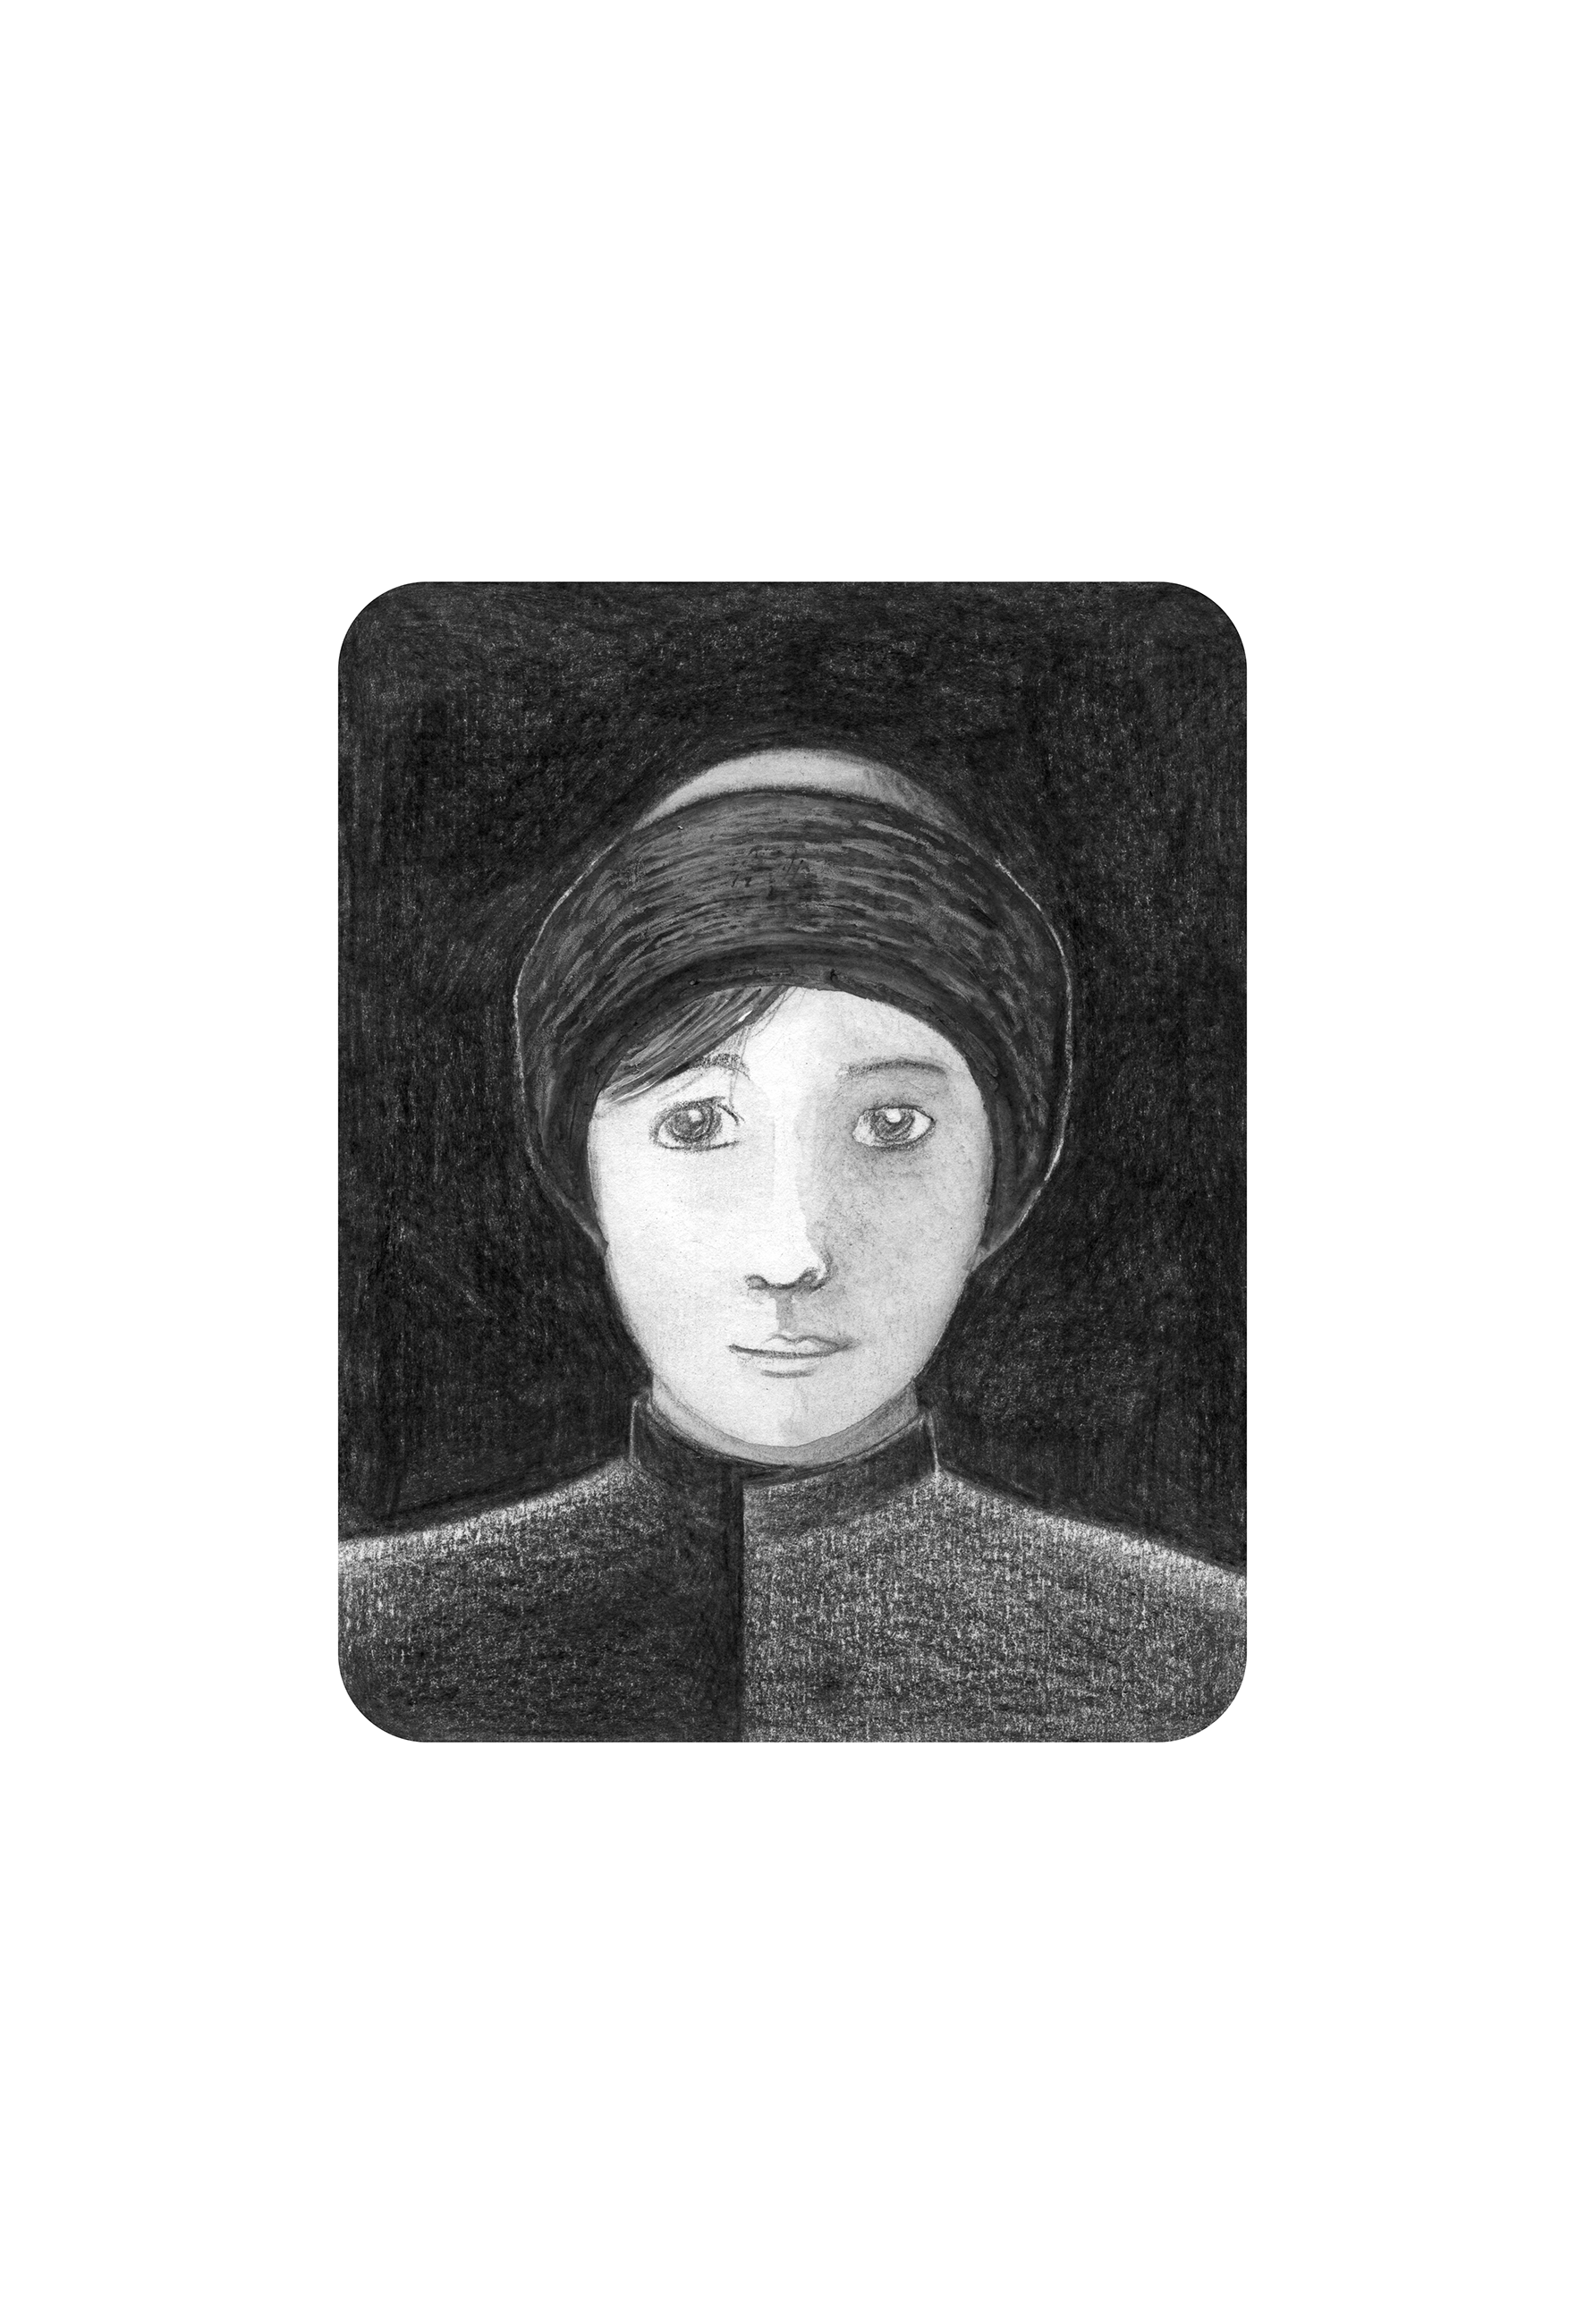
\includegraphics[width=5cm]{./images/PNLD0049-10.png}}

\subsection{Pós"-leitura \textsc{iii}}

\paragraph{Tema} Sociedade dos poetas vivos: a poesia como forma de expressão
juvenil.

\BNCC{EM13LP28}
\BNCC{EM13LP46}
\BNCC{EM13LP47}
\BNCC{EM13LP53}
\BNCC{EM13LP54}
\BNCC{EM13LGG603}

\paragraph{Conteúdo}
Apresentação aos alunos da possibilidade de se exprimir por meio de
versos, relembrando o poeminha redigido por Nikita, quando seu coração
estava transbordando de novos sentimentos.

\paragraph{Objetivos}
Introduzir alunos e alunas na escrita da poesia, incorporando noções de
rima, métrica e versificação e, mais que isso, aproximando essa forma
poética do mundo subjetivo do jovem e da cultura contemporânea.

\paragraph{Justificativa}
Na Rússia, desde a mais tenra infância, a criança é apresentada à poesia
e ao principal nome da literatura nacional: o poeta Aleksándr Púchkin
(1799-1837), que, entre tantas contribuições, consagrou o sistema
poético (sílabo"-tônico) usado até hoje no país. A poesia para os russos
talvez seja tão significativa como a música é para os brasileiros.
Assim, as experiências poéticas de Nikita podem ocorrer a qualquer jovem
russo contemporâneo, já que as crianças do país continuam a repetir e
decorar versinhos antes mesmo de saberem escrever. Não à toa surge na
velha casa a figura de Púchkin, no auge do amor de Nikita pela menina de
laço azul: ``Uma luz avermelhada iluminou as costas das poltronas de
couro, um canto de uma moldura dourada na parede e o busto de Púchkin
entre os armários''. (\textsc{tolstói}, 2021, p. 69)


\begin{figure}[ht!]
\includegraphics[width=\textwidth]{./images/PNLD0049-11.png}
\end{figure}

Apesar de o contato com a poesia ser menos intenso no Brasil, a ideia
aqui é que o professor proponha um exercício lúdico de criação,
possibilitando a identificação dos alunos e alunas com a arte poética,
que pode surgir em diversos contextos não tradicionais: \emph{slams},
letras de \emph{rap,} de sambas, \emph{posts} no \emph{Instagram}.

Propõe"-se, portanto, o trabalho com uma linguagem viva e dinâmica,
mostrando aos alunos que a poesia pode ser uma forma de se expressar no
mundo contemporâneo. Uma das mais importantes referências pedagógicas
reside no trabalho com as experiências pessoais dos educandos, suas
histórias de vida e impressões do mundo, seus desejos e anseios. Assim,
a poesia pode desempenhar um importante papel na transformação
individual e social do educando.

\paragraph{Metodologia}

Algumas atividades são recomendáveis antes da escrita poética. Sugerimos
a organização de um ou mais grupos que formarão a \emph{Sociedade dos
Poetas Vivos,} que pode ser orientada por estudantes de turmas mais
avançadas ou por professores. A dinâmica de trabalho poderá ser dividida
da seguinte forma:

\begin{enumerate}
\item
Pré"-escrita

Pesquisa sobre poesia russa e poesia em geral. Aqui, não se exige que
o estudante se debruce tanto sobre teoria da poesia, mas, sim, que ele
encontre poemas que o toquem e os compartilhe com a turma. Uma breve
biografia dos autores selecionados também será bem"-vinda. É desejável
--- mas não obrigatório, com vistas a não inibir --- que o estudante
discorra sobre o que o comove e como ele interpreta os poemas
escolhidos.

O educando do ensino médio, que pode já estar familiarizado com noções
de métrica e rima, com o verso branco e o verso livre, terá a
oportunidade de rever esses temas. O estudante não precisa se concentrar
apenas em poemas mais convencionais, pode pensar em letras de \emph{rap}
e de música em geral, tentando definir algumas características desses
textos (do ponto de vista da forma e do conteúdo).

\item
Escrita

A sociedade terá a função de suscitar a produção poética e poderá durar
por período indefinido. De início, é possível eleger temas e formatos
comuns, que serão apresentados e escolhidos em assembleia. A ideia de
estabelecer temas e formatos (haicais, sonetos, versos livres, poesia
concreta etc.) é interessante por possibilitar ao aluno experimentações
poéticas variadas. Também indicamos a leitura coletiva dos versos
produzidos, para que os colegas possam compartilhar suas criações e
ajudar uns aos outros.

Uma proposta para fortalecer o sentimento de grupo inclui a exibição do
filme \emph{A sociedade dos poetas mortos} (Dir. Peter Weir, 1989).
Conta a história de alunos de uma escola demasiadamente conservadora
que, em busca de liberdade de expressão artística e inspirados por um
novo professor de literatura, fundam um clube secreto para leitura de
poesia.
\end{enumerate}

\paragraph{Tempo estimado} Indefinido, podendo durar os três anos do
ensino médio.

\section{Atividades 2}

Orientações gerais para a utilização dos temas e conteúdos
presentes na obra, visando a uma abordagem interdisciplinar.

\paragraph{Tema} O contexto histórico de \emph{A infância de Nikita} nos últimos tempos de Rússia Imperial.

\BNCC{EM13LP01}
\BNCC{EM13LP25}
\BNCC{EM13LGG303}
\BNCC{EM13CHS101}
\BNCC{EM13CHS102}
\BNCC{EM13CHS201}

\paragraph{Objetivos}
Estabelecer a relação espaço"-tempo da narrativa com a história russa e
mundial no fim do séc. \textsc{xix}, lembrando aos educandos a questão da
servidão e da pós"-servidão na Rússia, para estabelecer semelhanças e
diferenças com a escravatura e sua abolição no Brasil.

\paragraph{Justificativa}
O contraste entre a Rússia e os principais países da Europa se enraizou
a partir das primeiras décadas do século \textsc{xix}. Na Europa Ocidental, o
processo de industrialização favorecia mudanças, como forte urbanização,
aumento da produtividade e divisão de trabalho, que alteraram desde os
meios de transporte até as relações comerciais, mas, na Rússia, o
cenário se estagnou: a monarquia continuava a ser absolutista e a base
econômica agrária, apoiada na chamada servidão dos camponeses.

Até a segunda metade do século \textsc{xix}, a sociedade russa era essencialmente
agrária. O país era governado por um regime autocrático, centralizado na
figura do tsar. Mais de 80\% da população era formada por camponeses
pobres, sujeitos à fome, à pobreza e ao analfabetismo. Com o
desenvolvimento industrial, muitos camponeses foram atraídos para as
cidades, formando uma camada de operários mal remunerados. Enquanto
isso, a burguesia industrial enriquecia, tornando mais evidentes as
desigualdades sociais na Rússia tsarista.

Publicado em sua forma integral em 1922, em Berlim, o relato de \emph{A
infância de Nikita,} que remonta à última década do século \textsc{xix},
entrecruza o histórico e o literário. A obra é resultado das memórias de
infância do escritor em uma província russa em Samara. O livro constitui
uma narrativa em que o tempo de enunciação se estabelece em um momento
muito importante da história russa: o fim, então recente, da servidão
(1861), o desenvolvimento da industrialização e os primeiros passos rumo
à Revolução de 1917.

Trata"-se de leitura aparentemente leve e fluida, mas favorável à
abordagem de assuntos nevrálgicos, como a cultura do favorecimento, a
presença dos agregados, a constante reverberação da servidão, etc. ---
revelando que algumas tradições culturais russas têm clara semelhança
com as brasileiras. Além disso, Aleksei Tolstói escreveu \emph{A
infância de Nikita} (1922) durante o período de emigração. Portanto,
embora ele tenha começado a novela depois de Revolução (1917) e
terminado no ano da criação da \textsc{urss} (1922), ela não reflete a realidade
soviética, trazendo muitos elementos que deixaram de existir no país: a
rígida instituição da família, os valores aristocráticos, a celebração
de datas religiosas, como Natal e Páscoa (proibidos após 1929), etc.

\paragraph{Metodologia}
Esta atividade pode ser iniciada explicando"-se o contexto russo do
século \textsc{xix}, quando a classe dirigente era composta da nobreza
proprietária de terras, que tinha servos e o poder de vendê"-los,
doá"-los, apostá"-los em jogo e até matá"-los. Os demais camponeses serviam
em terras pertencentes ao Estado, à família imperial ou à Igreja
Ortodoxa Russa. Era reduzido o número de mercadores e donos de
manufaturas.

\begin{figure}[ht!]
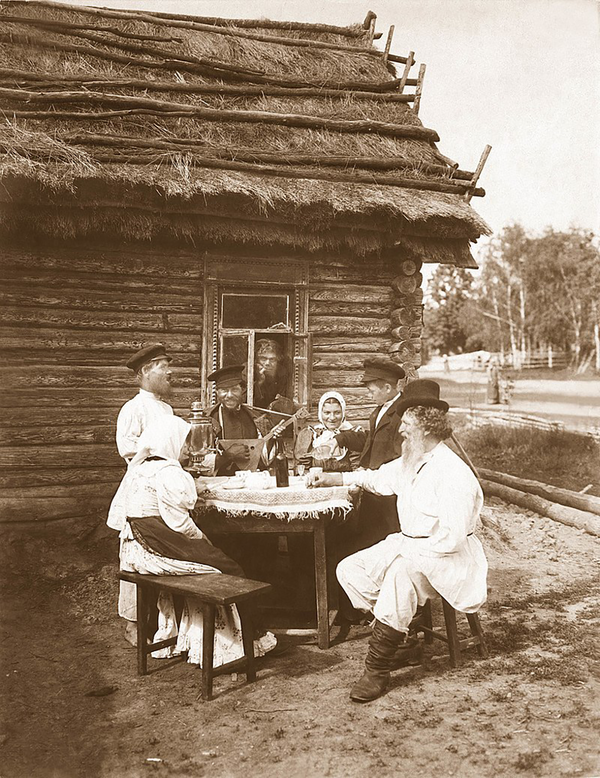
\includegraphics[width=\textwidth]{./images/PNLD0049-12.png}
\end{figure}

Em meados desse século, Napoleão \textsc{iii} aproximou"-se da Inglaterra,
apoiando"-a na Guerra da Crimeia (1854-1856) contra a Rússia, que saiu
derrotada dos conflitos. Quando estourou a guerra na península, a
coligação entre a Inglaterra, a França, o reino italiano do Piemonte e o
Império Turco"-otomano barrou o avanço dos russos sobre o mar Negro,
destruindo o exército do tsar em 1855. Assim, em 1856, o Tratado de
Paris terminou de vez com as pretensões russas de alcançar o
Mediterrâneo e afundou o país em uma crise. Acreditando que a concessão
de medidas libertárias ajudaria a reerguer o império russo da recessão
após a Guerra da Crimeia, o tsar Alexandre \textsc{ii} (que reinou entre 1855 e
1881) encenou a libertação dos servos das glebas em 1861:

\begin{quote}
Entretanto, a reação dos conservadores foi ferrenha e fez com que as
reformas saíssem atenuadas, quando não contraproducentes. Quando
finalmente foi promulgada a lei, em 1861, o camponês não se tornava
completamente livre, mas, sim, membro de uma comunidade responsável
coletivamente pelo pagamento de uma série de obrigações (dívidas) ao
senhor territorial. Na realidade, a valorização da terra fazia com que
essas dívidas crescessem continuamente, dificultando cada vez mais a
redenção efetiva. Além disso, o abandono da comunidade rural era
impedido pelo sistema de posse coletiva, tornando a libertação uma
medida irrisória: o novo sistema criara males talvez maiores que o
antigo, o que foi confirmado pela baixa do padrão de vida no campo. Está
aí esboçado o quadro em que se projetaram sucessivamente ondas de
descontentamento e repressão, até os primórdios da revolução de 1905.
(\textsc{bernardini}, 2018 p. 176)
\end{quote}

\begin{figure}[ht!]
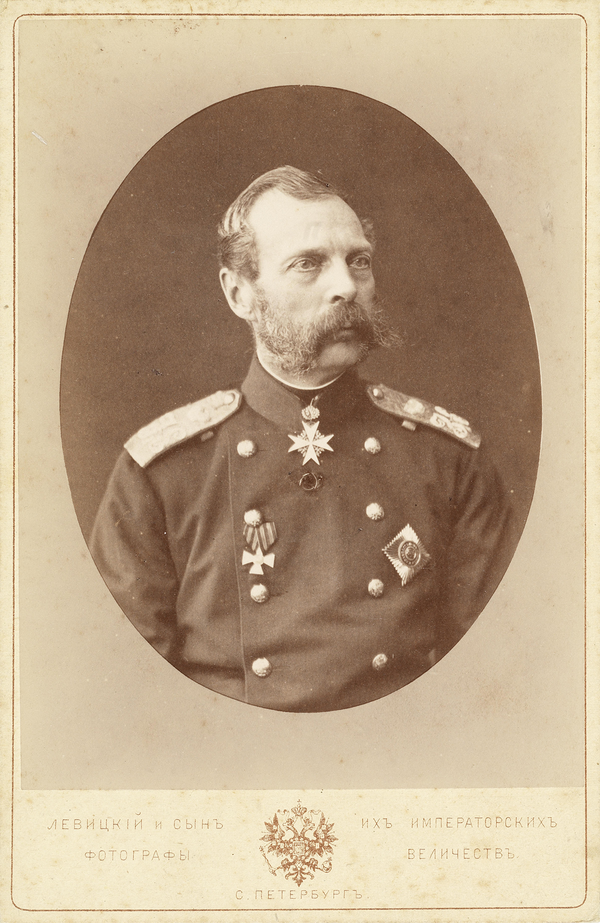
\includegraphics[width=\textwidth]{./images/PNLD0049-06.png}
\end{figure}

Assim, em março de 1881, depois de sofrer diversos atentados, Alexandre
\textsc{ii} morreu em consequência de um ataque do grupo Vontade do Povo. Até
1905, quando uma nova derrota russa, dessa vez para os japoneses,
resultou em séria revolta contra o tsar Nicolau \textsc{ii} (que reinou entre
1894 e 1917), a situação da servidão, na prática, sofreu poucas
alterações, assim como a da monarquia absolutista, da nobreza e da
Igreja Ortodoxa Russa. Mas, do ponto de vista econômico, ocorreram
mudanças importantes entre os anos 1860 e 1890, principalmente com a
entrada de capital estrangeiro, que financiou a criação de grandes
empresas. O Estado construiu nessa época ferrovias ligando Moscou às
províncias e estimulou as indústrias de base, criando polos industriais,
como o de São Petersburgo, capital do país na época.


\marginnote{\footnotesize\textbf{PARA LER}\\ Populismo no país adotou estratégias terroristas;
movimento foi responsável por atentado que matou o tsar Alexandre \textsc{ii}
(\emph{Folha de S. Paulo}, 10/07/20718):\\
\url{https://bit.ly/3ei5Iev}
}

Quando Alexandre \textsc{iii} (que reinou de 1881 a 1894) subiu ao trono, se
iniciaram os ``anos crepusculares'' da Rússia: os chamados
ocidentalistas propunham reformas radicais e acreditavam que a mudança
econômica e social segundo modelos ocidentais era o único meio de
atingir a industrialização que se desenvolvia nos grandes centros
europeus e ampliava o proletariado urbano. Ao mesmo tempo, o país
desenvolvia o imperialismo nos Bálcãs, além de uma identificação
cultural com os povos eslavos que mais tarde foi chamada de
pan"-eslavismo.

Neste ponto, partimos para a atividade com os alunos:

A sala pode ser dividida em grupos de pesquisa que apresentarão
paralelos entre ``A Servidão na Rússia e sua Abolição'' e ``A Escravidão
no Brasil e sua Abolição''. Ao fim da apresentação, dois grupos, com
auxílio do educador, devem tentar defender seus pontos de vista sobre a
existência ou não de grandes diferenças entre servidão e escravidão,
tendo em mente ainda os conceitos de ``situação análoga à de
escravidão'' e ``escravidão moderna''. Uma sugestão de texto para
preparar este debate é: ``Por que a servidão russa não era exatamente
escravidão?''.

\marginnote{\footnotesize\textbf{PARA VER}\\ ``Servo'' (\emph{Kholop}/ \emph{Son of a rich}, \textsc{rus}, 2019, Comédia): um mauricinho ultrapassa todos os limites e seu pai
resolve colocá"-lo na linha mandando"-o de volta a tempos remotos e
transformando"-o em servo.}

Partindo para o livro \emph{A infância de Nikita,} os alunos poderão
trabalhar seus indícios temporais. Um dos elementos que poderá ser
apontado é a divisão de classes de fins do século \textsc{xix}. O protagonista
pertence à nobreza decadente, a uma família proprietária de terras, ao
passo que seu melhor amigo, Michka Koriachónok, pertence à massa
camponesa. O fato de Nikita ser oriundo de uma nobreza decaída explica o
contato que tinha com os criados da casa, embora a hierarquia não fosse
rompida. Tal fato pode ser localizado em diversos trechos, como a festa
de Natal que a mãe organiza e da qual participam as crianças menos
abastadas dos agregados. A existência de um preceptor em casa, como
supracitado, era privilégio de famílias nobres ou enriquecidas, que
costumavam educar os filhos, quando pequenos, dessa maneira. É
esclarecedora a conversa da mãe de Nikita com a amiga que a fora visitar
na época de Natal:

\begin{quote}
--- Não e não, Aleksandra Leóntievna --- bramia ela ---, eduque seu
filho em casa. No ginásio há tantas desordens horrorosas que minha
vontade é pegar com as próprias mãos o diretor e o pôr porta afora\ldots{}
Víktor --- exclamou repentinamente ---, não é de sua conta o que sua mãe
está dizendo sobre adultos, você deve respeitar os superiores.
(\textsc{tolstói}, 2021, p. 57)
\end{quote}

É digno de nota aqui que, nem mesmo seu pertencimento a uma nobreza
decadente --- em certo ponto do livro descobrimos que a família devia
três meses de salário ao preceptor --- muda a condição social da
família.

Outro ponto a ser apontado na leitura da novela são as festas
religiosas tradicionais na Rússia Imperial: Natal e Páscoa. A
religiosidade em si não é explorada de maneira marcante na obra de
Tolstói, mesmo com a enorme importância da Igreja Ortodoxa Russa --- até
1861, servos eram considerados ``gente'', e não ``objetos'', apenas se
batizados. Em todo caso, a árvore de Natal exerce um efeito quase mágico
na obra (é quando Nikita dá seu primeiro beijo), ao passo que na União
Soviética, depois de 1929, a data foi eliminada, junto com outros
feriados religiosos, do calendário oficial. Mesmo sem sentido religioso,
a ``árvore de Natal'' continuou a ser montada e passou a ser ligada à
festividade do \emph{Réveillon}, virando ``árvore de Ano"-Novo''.

\begin{figure}[ht!]
\includegraphics[width=\textwidth]{./images/PNLD0049-13.png}
\end{figure}

Após o fim da \textsc{urss}, a população russa, em geral bastante religiosa,
voltou a comemorar abertamente as festas da Igreja. O Natal russo é
comemorado em 7 janeiro, seguindo o velho calendário juliano (o
calendário gregoriano só foi adotado em 1918), mas a celebração ortodoxa
mais importante do país é certamente a Páscoa, período, por sinal, em
que Nikita vai à igreja da aldeia e passa um dia brincando com os
vizinhos.

\marginnote{\footnotesize\textbf{PARA LER}\\ ``Papai Noel Russo usa casaco de peles e trenó com
cavalos'' -- \emph{Folha de S. Paulo} (08/07/2018).
\url{https://www1.folha.uol.com.br/esporte/2018/07/falando-russo-papai-noel-usa-casaco-de-peles-e-treno-com-cavalos-na-russia.shtml}}

\paragraph{Tempo estimado} Quatro a cinco aulas de 50 minutos.

\subsection{Pré"-leitura}

\paragraph{Tema} Cineclube russo: \emph{O Pracinha de Odessa}.

\BNCC{EM13LP46}
\BNCC{EM13LP01}
\BNCC{EM13LP22}
\BNCC{EM13CHS201}

\paragraph{Conteúdo}
Exibição do filme \emph{O Pracinha de Odessa} (dir. Luis Felipe Labaki,
2013), disponível gratuitamente no canal da Universidade de São Paulo no
YouTube, seguida de rodadas de discussão.

\paragraph{Objetivos}
Aproximar o educando do ofício do tradutor por meio das memórias de
Boris Schnaiderman, expoente da difusão de literatura russa no Brasil e
da prática da tradução direta. Além de fornecer um vislumbre da
profissão, o filme familiariza o aluno com o período de escrita do livro
de Tolstói (início do século \textsc{xx}) e o de ação do livro (final do século
\textsc{xix}), tocando em eventos importantes que ocorreram na Rússia.

\paragraph{Justificativa}
Nascido na Ucrânia, então parte do império russo, o tradutor, escritor e
fundador da cátedra de russo da Universidade de São Paulo Boris
Schnaiderman (1917-2016) emigrou com a família para o Brasil em 1924. Em
seu curto período na terra natal, ele teve experiências que o marcaram
por toda a vida. Essas memórias são recontadas neste curta"-metragem
realizado por Luis Felipe Labaki, tradutor e cineasta que usou em sua
montagem elementos do cinema russo do início do século \textsc{xx}. O filme traz,
em primeiro lugar, a chance de os alunos conhecerem a trajetória de
Schnaiderman, que definiu os rumos da tradução moderna do russo no
Brasil. Além disso, poderão aprofundar"-se no contexto histórico de
\emph{A infância de Nikita}, aproximar"-se da cultura russa e vislumbrar
possibilidades profissionais.

\begin{figure}[ht!]
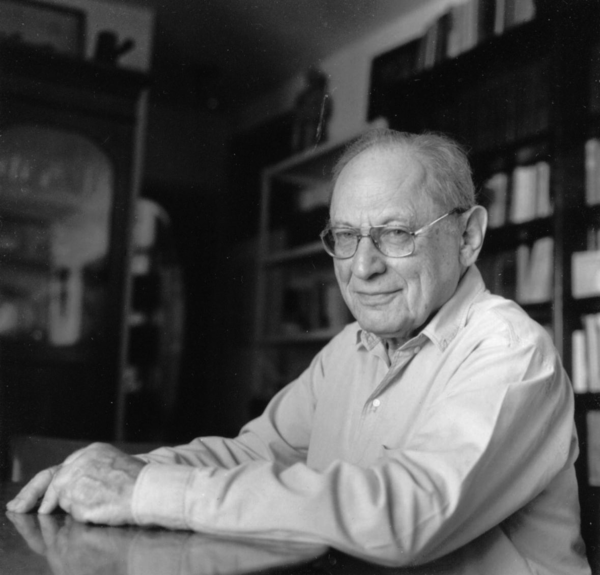
\includegraphics[width=\textwidth]{./images/PNLD0049-14.png}
\end{figure}

\paragraph{Metodologia}
Como se trata de um filme de 22 minutos, não é necessário organizar uma
sala de exibição, sendo possível exibir o título na própria sala de aula
com o devido equipamento. O ideal é que o educador acompanhe a exibição,
depois da qual poderá ser organizado um debate. É desejável que os
alunos tenham um caderno de anotações para a tarefa, registrando
comentários, questões e pontos que julguem importantes. A atividade pode
ser concluída com a elaboração de uma redação sobre o ofício do
tradutor, compreendido como um arauto cultural. Além disso, é possível
pensar em como o jovem diretor reorganizou as memórias de Schnaiderman
em primeira pessoa e como intercalou reminiscências literárias com
eventos históricos. Uma terceira alternativa seria abrir a discussão
para as profissões e aspirações dos estudantes.

Outras questões podem ser colocadas: Os educandos conhecem o filme
\emph{O Encouraçado Potemkin} (1925), cujas gravações o tradutor lembra
ter presenciado nas escadarias de Odessa? E conhecem o episódio
histórico de que trata esse filme? O educador, então, pode falar um
pouco sobre a importância de Serguei Eisenstein para a história do
cinema e contar sobre o motim organizado pela tripulação do navio
Potemkin, em junho de 1905, pelas condições desumanas de trabalho.

\paragraph{Tempo estimado} Duas a quatro aulas de 50 minutos.


\subsection{Leitura}

\paragraph{Tema} A mulher na sociedade russa do século \textsc{xix}.


\bnccativividadesleitura
\BNCC{EM13LP01}
\BNCC{EM13LP20}

\paragraph{Conteúdo}
A familiarização do jovem leitor com a chamada ``questão feminina'' e
seus desenvolvimentos no século \textsc{xix} na Rússia.

\paragraph{Objetivos}
Abranger uma diversidade de temas e de contextos sociais, culturais e
históricos que se mostra de suma importância para a vida de mulheres.
Destacar a participação da mulher em diferentes atividades e espaços de
poder, conferindo"-lhe visibilidade e protagonismo social.

\paragraph{Justificativa}
Nikita vivia dentro de uma família tradicional e, além disso,
aristocrática, apesar de um tanto instável em vários sentidos, inclusive
financeiro. Seu pai, visivelmente, tinha compulsão por gastar enormes
somas em mercadorias inúteis e era sua esposa, Aleksandra Leóntievna,
quem fornecia o ponto de equilíbrio à vida e às finanças da família, mas
o fazia entre quatro paredes. A atividade é relevante para que
estudantes reflitam: Qual era a posição da mulher na sociedade de então
e por quais mudanças ela passará?

\paragraph{Metodologia}
A atividade pode se iniciar com um breve panorama das discussões e
conquistas russas quanto à emancipação da mulher no século \textsc{xix}. Nesse
período, o aumento da indústria caseira europeia teve um grande impacto
no papel das mulheres, já que a economia doméstica se caracterizava pela
combinação entre agricultura e manufatura (apenas a exploração agrária
era insuficiente para sustentar uma família). Assim, como escreve Wendy
Goldman:

\begin{quote}
O desafio plebeu à autoridade patriarcal desde baixo se combinava com o
desafio filosófico desde cima, uma vez que debates sobre a mulher e a
família atraíam pensadores livres do Iluminismo. Embora as filosofias
não estivessem preocupadas diretamente com a libertação das mulheres,
elas moldavam a discussão do papel das mulheres de uma maneira
totalmente nova ao abri"-la para questões de diferença de gênero e para o
potencial de igualdade das mulheres. (\textsc{goldman}, 2014, p. 37)
\end{quote}

Mas, enquanto muito do pensamento filosófico na época era novo, as
conclusões dos filósofos continuavam a ser conservadoras. Por exemplo,
Diderot, ao mesmo tempo que criticava instituições e costumes que
limitavam as mulheres, acreditava que estas eram propensas, como um
defeito de nascença, à histeria e incapazes de manter concentração
mental.

As expressões limitadas de feminismo contidas na Revolução Francesa
demonstraram que as demandas pela emancipação da mulher não poderiam ser
realizadas enquanto o lar desempenhasse papel central na produção.

\begin{quote}
Em seus momentos mais radicais, os filósofos questionaram a
superioridade ``natural'' do homem e defenderam mais oportunidades
educacionais para as mulheres. Voltaire e Diderot questionaram a
desigualdade legal e Montesquieu defendeu que o caráter feminino não era
inato, mas sim o resultado de uma educação ruim e de oportunidades
limitadas (\textsc{goldman}, 2014, p. 38)
\end{quote}

Nesse sentido, a Rússia esteve
entre os países pioneiros ao permitir que pessoas do sexo feminino
tivessem suas próprias instituições de ensino superior (já que elas não
podiam frequentar as existentes). Em 1869 foram fundados os primeiros
cursos superiores para mulheres, os Cursos Lubianskie de Moscou e os
Cursos Alartchinskie de São Petersburgo, aqui seguidos dos Cursos
Vladimirskie (1870), para homens e mulheres, dos Cursos Guerrier (1872),
em Moscou, e dos Cursos Bestujev (1878). Isso permitiu pela primeira vez
que cientistas, professoras rurais e revolucionárias obtivessem formação
superior no país. Vale lembrar que, na década de 1920, quando Virginia
Woolf foi convidada a palestrar em duas faculdades inglesas exclusivas
para mulheres (o que deu origem ao ensaio \emph{Um teto todo seu}), ela
relatou que, refletindo sobre o colóquio, resolveu se sentar no gramado
de Oxbridge e foi de lá expulsa por um bedel horrorizado: ``Ele era um
bedel; eu era uma mulher. Aqui era o gramado; ali estava o caminho.
Somente os estudantes {[}do sexo masculino{]} e os professores eram
admitidos aqui''. (\textsc{woolf}, 2014, p. 15) Só em outubro de 1920 as mulheres
passaram a ser admitidas formalmente em Oxford.

A chamada ``questão feminina'' passou a povoar o pensamento e a cultura
russos em meados do século \textsc{xix}. Manifestações de autoras russas a
respeito da condição feminina começaram a se evidenciar em escritos das
décadas de 1830 e 1840, deixando um legado significativo.

\begin{quote}
Os avanços dos sociais"-democratas europeus na questão da mulher
certamente influenciaram suas contrapartes russas, mas os círculos
progressistas na Rússia há tempos defendiam as ideias de união livre e
de igualdade das mulheres. A ênfase de George Sand no amor e nos
imperativos emocionais do coração encontrou um público entusiasta entre
a aristocracia russa na década de 1830, e as defensoras da educação
feminina nos anos 1850 reiteraram muitos debates europeus sobre o
potencial das mulheres. (\textsc{goldman}, 2014, p. 64)
\end{quote}

Os anos 1850 podem ser considerados um marco na primeira onda da luta
pela emancipação feminina. O movimento avançou durante a segunda metade
do século \textsc{xix} e atingiu seu ápice entre as Revoluções de 1905 e 1917,
estendendo"-se até 1920.

\begin{quote}
As chamadas ondas do feminismo russo, desde suas raízes no século \textsc{xix}
até as transformações ocorridas ao longo do século \textsc{xx}, são muito
peculiares. Elas incluem mulheres da aristocracia, de instituições
filantrópicas, da \emph{intelligentsia}, marxistas, das alas liberal,
radical etc. --- o movimento de mulheres da Rússia se difere das
conquistas das mulheres ocidentais dentro do liberalismo, que
reivindicavam a igualdade de direitos em relação aos homens, sem propor
uma mudança abrupta nos padrões sociais, enquanto na Rússia pré e
pós"-revolucionária a transmutação do papel e dos costumes impostos à
mulher era crucial. (\textsc{schneider}, 2017, p. 14)
\end{quote}

Assim, a representação feminina na literatura russa é uma fonte de
estudo valiosíssima para se compreender a situação da mulher antes de
sua emancipação em várias partes do mundo. A mãe de Tolstói, Aleksandra
Leontievna, era escritora e, depois de deixar o pai do menino para viver
com Aleksei Bostrom, dedicou"-se assiduamente à literatura, publicando
dez livros de prosa para adultos, crianças e jovens, além de diversos
artigos em jornais e revistas --- chegando até mesmo a conhecer Górki.
No livro, a mãe de Nikita, homônima à de Tolstoi, também compartilha do
gosto pelas letras, sempre inclinada sobre livros:

\begin{quote}
A mãezinha inclinou a cabeça sobre o livro, os cabelos dela eram
cinzentos, finos e se enrolavam na têmpora, onde havia uma marca de
nascença parecida com um grão de cevada. De tempos em tempos, cortava as
folhas com a agulha de tricô. O livro tinha capa cor de tijolo. O
armário do escritório do pai estava cheio de livros como aquele, todos
se chamavam \emph{Mensageiro da Europa} {[}revista liberal
político"-literária{]}. É surpreendente como adultos gostam de tudo o que
é tedioso: ler um livro assim é como empilhar tijolos. (\textsc{tolstói}, 2021,
p. 45)
\end{quote}

Vale lembrar que o Instituto Smólny de Donzelas Nobres, primeira
instituição de ensino feminino do país e primeira estatal do gênero na
Europa, foi fundado em 1764 e era frequentado por garotas dos seis aos
dezoito anos de idade. Assim, o país foi pioneiro também na educação
fundamental e média feminina por meio do decreto de fundação da
instituição de Catarina, a Grande, que assinalava o objetivo de
``entregar ao Estado mulheres educadas, boas mães, membros úteis da
família e da sociedade''.

\begin{figure}[ht!]
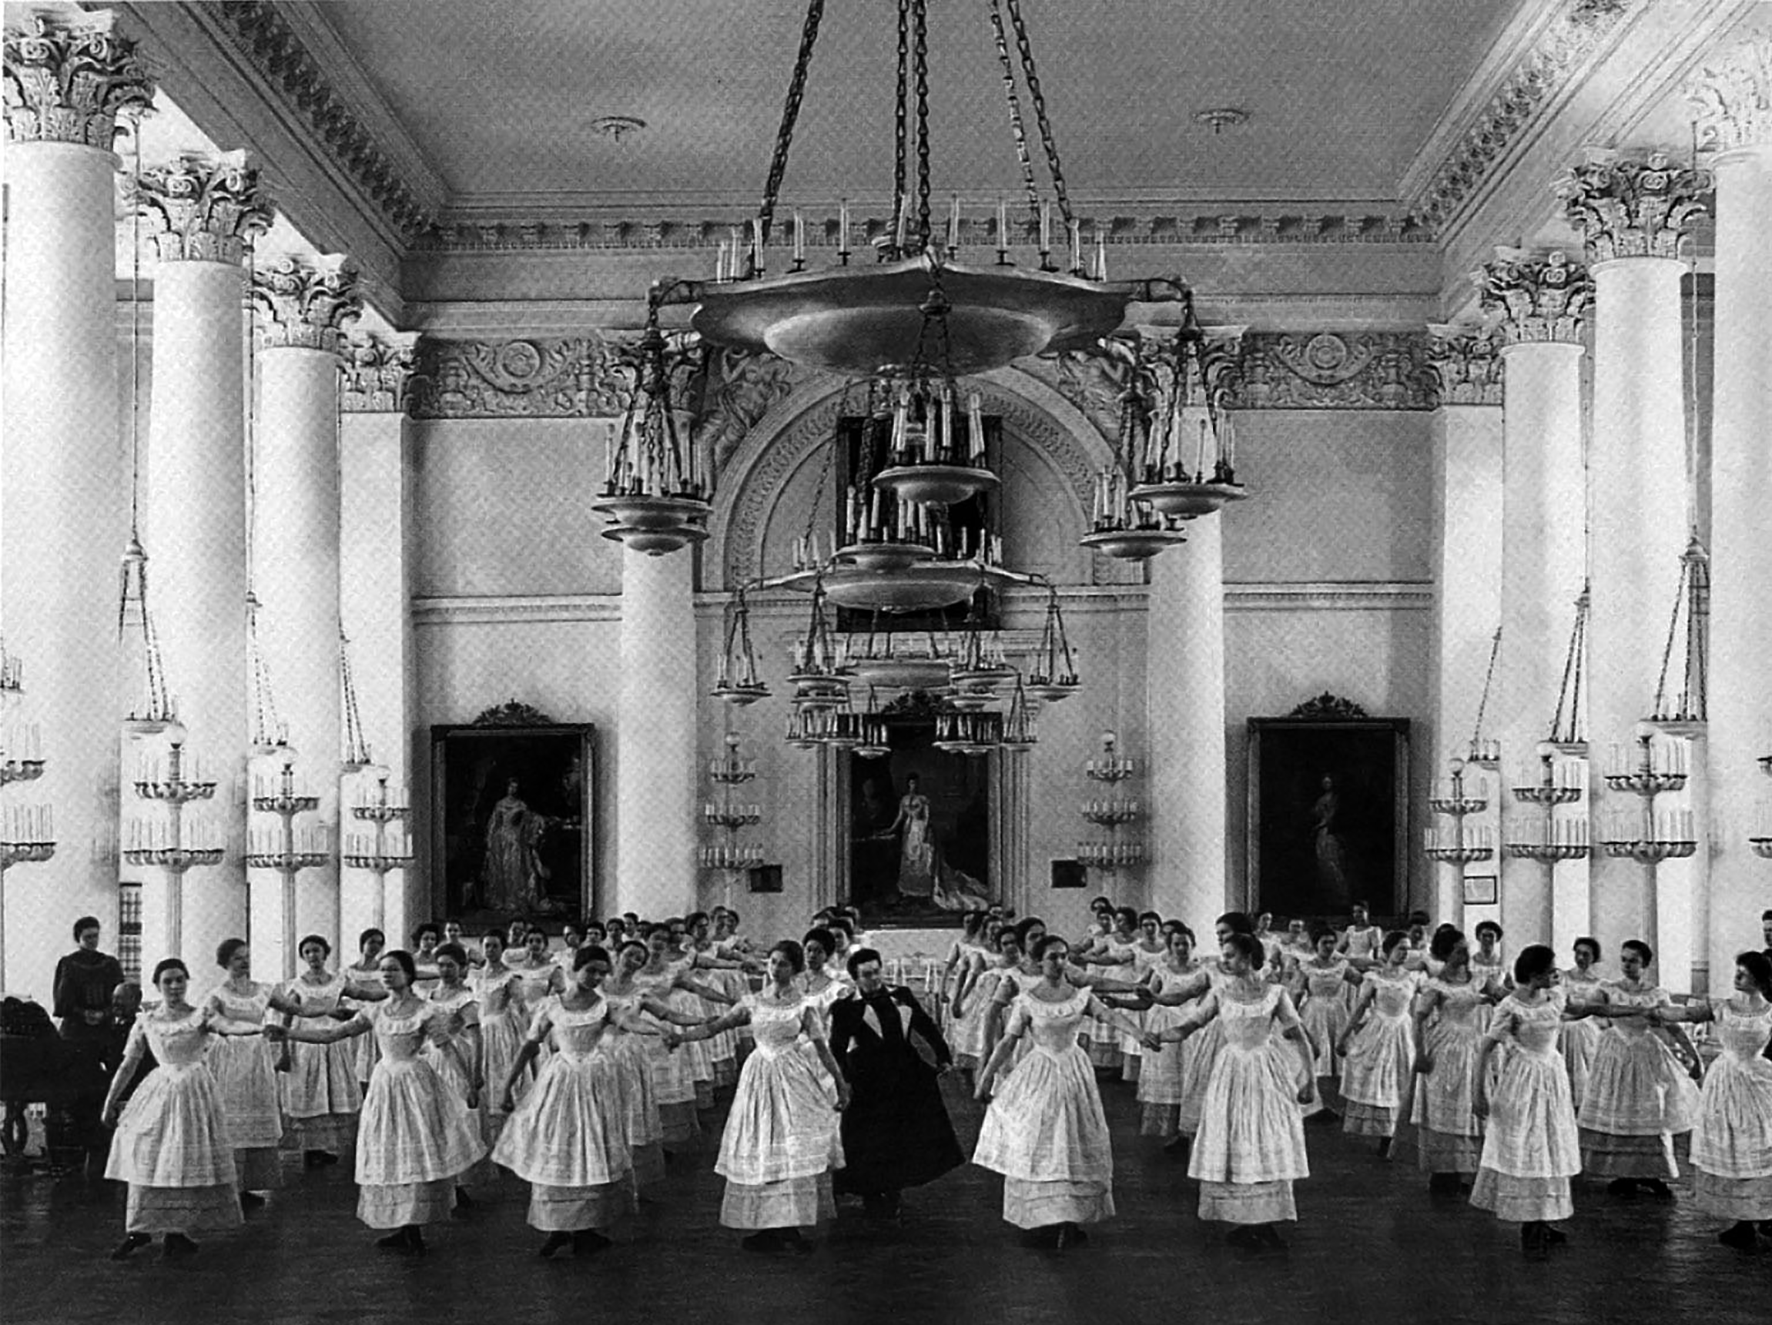
\includegraphics[width=\textwidth]{./images/PNLD0049-15.png}
\end{figure}

Nesta fase da atividade, os educandos deverão se dividir em grupos que
pesquisarão a condição da mulher no século \textsc{xix} no Brasil e na Rússia
para apresentarem seminários aos colegas. Cada um dos grupos, além de
apresentar um panorama da condição da mulher e das discussões em voga no
período escolhido, terá que trazer nomes de figuras femininas que tenham
sido expoentes na literatura, nas artes, nas ciências e nas camadas
intelectual e política da época.

\paragraph{Tempo estimado} Uma aula de 50 minutos para cada dois grupos de
apresentação e tempo adicional para debates.

\subsection{Pós"-leitura}

\paragraph{Tema} Ciências humanas -- geografia: a região de Samara e o rio Volga.

\BNCC{EM13LP01}
\BNCC{EM13CHS101}
\BNCC{EM13CHS102}
\BNCC{EM13CHS206}
\BNCC{EM13CHS106}

\paragraph{Conteúdo}
Localização, pontos de interesse e importância da região de Samara e do
rio Volga para a Rússia.

\paragraph{Objetivos}
Familiarização do educando com o espaço geográfico em que ocorre a obra,
caracterizando e analisando sua importância histórico"-econômica.

\paragraph{Justificativa}
As relações do homem com a natureza têm enorme importância no livro
\emph{A infância de Nikita,} que destaca vários elementos, como o rio
Volga (Samara, onde fica a aldeia em que se passa o livro, fica na
região do Volga). Valiosíssimo para a Rússia, o Volga, com seus 3688~km,
é o mais longo rio da Europa e também o maior do
continente em caudal (volume/unidade de tempo) e na área de bacia
hidrográfica. O educando é capaz de apontar a localização da região de
Samara e do rio Volga no mapa? E ir mais além, discorrendo sobre a
história e importância econômica e cultural do rio para a Rússia?

\begin{figure}[ht!]
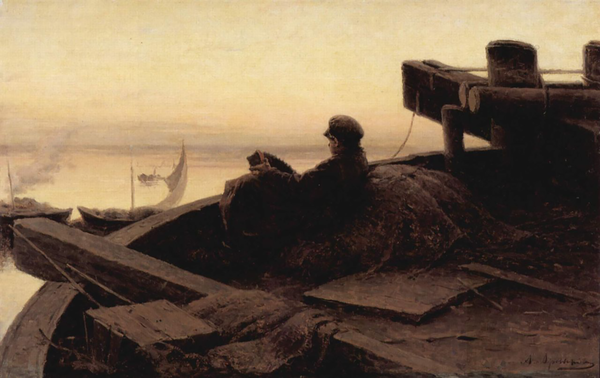
\includegraphics[width=\textwidth]{./images/PNLD0049-07.png}
\end{figure}

\paragraph{Metodologia}
Leia com os educandos as páginas 92 a 95 da obra. Neste trecho, Nikita
desenha o mapa da América do Sul a pedido da mãe --- que queria que ele
deixasse de fazer ``figuras bobas'' --- e conduz ``o rio Amazonas para o
lado errado, passando pelo Paraguai e pelo Uruguai para desembocar na
ilha da Terra do Fogo''. (\textsc{tolstói}, 2021, p. 92) Acontece que Nikita mora
próximo a um afluente, na região de Samara, do Volga, rio
importantíssimo para o país por suas dimensões e localização. Nikita,
como vemos desde o início da história, é um menino sonhador e desligado,
e não é dos estudantes mais aplicados, para dizer o mínimo. Aqui,
iniciaremos a atividade pedindo aos alunos que apontem no mapa da Rússia
esses dois pontos: o rio Volga e a região de Samara. É possível que não
consigam realizar a atividade de primeira. Pode"-se, então, aproveitar
para trabalhar com eles o mapa: tanto o russo --- apontando e deixando
que eles identifiquem a capital, Moscou, assim como a ex"-capital, São
Petersburgo, e outras cidades importantes, como Ekaterimburgo, ou os
montes Urais, que convencionalmente definem a fronteira entre Ásia e
Europa ---, como o europeu. Para complementar a atividade, sugerimos que
os educandos se dividam em grupos para pesquisar sobre Samara e o rio
Volga e discorrer sobre eles em uma aula posterior. Quais as atividades
desenvolvidas na região? Qual sua importância econômica?

\paragraph{Tempo estimado} Duas a três aulas de 50 minutos.

\section{Para aprofundar}

Aleksei Nikoláievitch Tolstói
(1883-1945) foi um dos principais escritores do período soviético,
aclamado pela crítica e pelo público. Um aristocrata \emph{déclassé}
típico das últimas décadas do império Romanov, o ``Conde Vermelho'',
como ficou conhecido, estabeleceu uma nova vertente literária durante a
construção da Rússia soviética, a do ``romance épico'', dentro do
realismo socialista.

\begin{figure}[ht!]
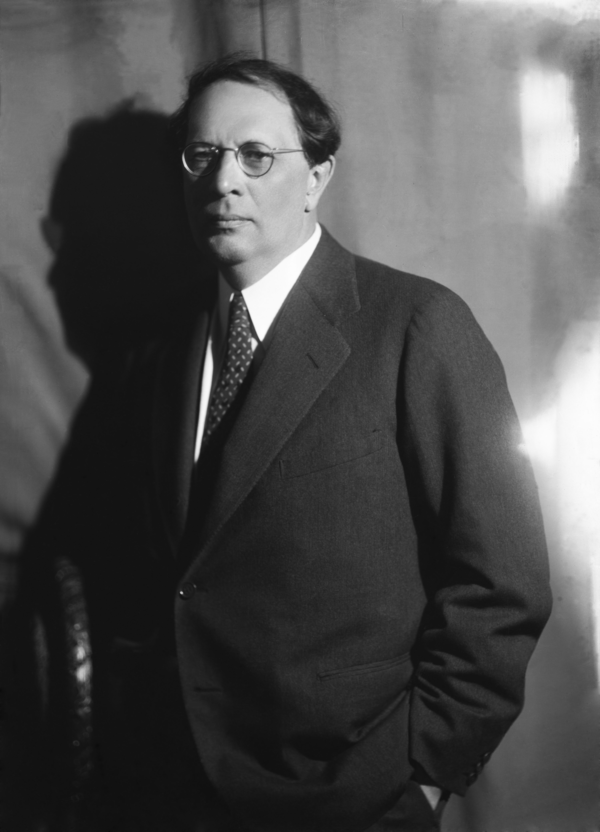
\includegraphics[width=\textwidth]{./images/PNLD0049-03.png}
\end{figure}

Apesar do sobrenome compartilhado com uma linhagem de aristocratas que
foram também grandes escritores, como Lev Tolstói e Aleksei
Konstantínovitch Tolstói (1817-1875), o ``Conde Vermelho'' levou uma
vida de classe média, crescendo em uma aldeia nos arredores de Samara e,
posteriormente, na própria cidade de Samara, mil quilômetros a leste de
Moscou.

No relato oficial, a mãe de Aleksei, Aleksandra Leôntievna (1854-1906)
deixou o pai dele, conde Nikolai Aleksаndróvitch Tolstói (1849-1900),
logo antes de o menino nascer, casando"-se com Aleksei Apollónovitch
Bostrom (1852-1921), um proprietário de terras empobrecido. Aleksei
levou o sobrenome do padrasto até os 16 anos de idade, quando sua mãe
iniciou o processo para alterá"-lo. Seu título de nobre e o sobrenome
Tolstói foram contestados posteriormente por figuras como Ivan Búnin
(1870-1953), Nina Berbérova (1901-1993) e Roman Gul (1896-1986).

Na infância, Aleksei fez um
colégio comum e de lá foi para a Faculdade Técnica de São Petersburgo,
com o intuito se tornar engenheiro. Durante a Primeira Guerra Mundial,
porém, foi correspondente e viajou entre França e Inglaterra em
1916. Entre os emigrados russos,
havia milhares de nobres decadentes que tinham crescido na pobreza e
estudado Marx na universidade ou até no ensino médio. Mas relativamente
poucos retornaram a sua terra natal nos anos 1920, como Aleksei Tolstói
o fez. Ao mesmo tempo, membros da mais alta nobreza, como o príncipe
Dmítri Sviatopólsk"-Mirsk, crítico e historiador literário, ou o Conde
Ignátiev, não só retornaram à Rússia, como se tornaram comunistas antes
de voltar. Por outro lado, os camponeses e trabalhadores das fábricas
que lutaram com o Exército Branco da Sibéria e emigraram para os \textsc{eua},
por exemplo, nunca quiseram retornar e se tornar cidadãos soviéticos.

Tolstói deixou a Rússia durante uma torrente de emigração do Exército
Branco e já era um escritor de considerável renome, tanto na ficção como
no jornalismo. Maksim Górki tinha seus textos satíricos sobre a
deterioração moral e cultural da nobreza russa em alta conta, e escreveu
a alunos da Escola Russa Social"-Democrata, em Bolonha: ``Prestem atenção
ao novo Tolstói, Aleksei, sem dúvida um escritor importante e poderoso
que descreve com uma precisão implacável a decadência psicológica e
econômica da nobreza contemporânea''. (\textsc{tolstói}, 1958)

Tolstói escreveu um número nada desprezível de obras voltadas para a
infância e a adolescência, como, por exemplo, \emph{Aelita} (1923),
romance de ficção científica, \emph{A chavezinha dourada, ou as
aventuras de Buratino} (1936)\emph{,} adaptação de \emph{Pinóquio}, de
Carlo Collodi, e muitos contos maravilhosos.

Aleksei Tolstói começou a publicar \emph{A infância de Nikita} em Paris
(1920), nos números 2, 3, 4, 5 e 6 da revista infantil de russos
emigrados \emph{Varinha verde} (\emph{Zeliónaia pálotchka}). No entanto,
o livro só saiu integralmente em Berlim pela editora Guelikon, em 1922,
sob novo título: \emph{Novela sobre muitas coisas maravilhosas}
(\emph{Póvest o mnóguikh prevoskhódnykh veschákh}). Títulos desse tipo
estavam em voga na Europa, mas na União Soviética o livro voltou a se
chamar \emph{A Infância de Nikita}. (\textsc{mountian}, 2021, Paratexto)

Em 1918, Aleksei Tolstói foi de Moscou para Odessa, acompanhado de sua
esposa Natália Krandriévskaia e de seu primogênito Nikita, que tinha
então um ano de idade. Depois, vivendo em Paris, envolveu"-se em círculos
aristocráticos de \emph{émigrés,} sendo considerado naquele momento o
grande literato russo, chefe da seção de literatura da revista de russos
emigrados \emph{Griadúschaia Rossia}.

Tolstói passava por sérios problemas financeiros e políticos quando
começou a publicar \emph{A infância de Nikita,} mudando"-se para Berlim
com a promessa de dirigir uma revista literária independente e
apolítica.

O autor tinha conflitos com tendências leninistas, mas apoiava a ideia
de um novo governo. O desejo de retorno à Rússia é perceptível na
novela, ``embora seu conteúdo se afaste, principalmente nos capítulos
publicados em Paris, das tendências pedagógicas que surgiram na Rússia
proletária de então'', como nota Mountian (2021, Paratexto).

Um aspecto de Tolstói que se refletiu no jornalismo que ele praticou
durante a Primeira Guerra e, mais tarde, na Segunda, assim como na
primeira parte de seu romance panorâmico \emph{O caminho dos tormentos,}
foi seu patriotismo arraigado e seu desejo de unidade da sociedade russa
--- que estava dividida em facções, face à terrível ameaça de uma
invasão alemã. Ele acreditava que a guerra, de alguma maneira, tiraria a
Rússia do beco sem saída em que se encontrava com os conflitos entre o
governo e as classes educadas.

Tolstói recebeu com entusiasmo a Revolução de Fevereiro de 1917. Ele
interpretou os eventos de então como o levante de uma nação inteira
contra um regime antiquado e prejudicial. Nesse sentido, estava em
consonância com a grande maioria das classes educadas da Rússia. Mas sua
reação à Revolução de Outubro de 1917, liderada por Lênin, foi muito
diferente. Tolstói colocou"-se, sem sombra de dúvida, ao lado dos
oposicionistas ativos contra uma ditadura comunista. Um conto intitulado
\emph{Em um delírio} reflete seus pontos de vista naquela época. Ele não
partiu ao autoexílio apenas para ter uma vida mais confortável naqueles
tempos turbulentos, mas também porque se opunha radicalmente aos
princípios e práticas dos seguidores de Lênin.

Um biógrafo de Aleksei Tolstói, no final dos anos 1940, tentou
justificar o retorno do escritor patriota à Rússia como um
reconhecimento do conde de que o regime de Lênin vencera e fora aceito
como governo nacional. Mas há outras nuances. Um escritor sempre terá
mais dificuldade de se ajustar ao exílio do que, por exemplo, um
engenheiro ou um químico, pois ele perde seu papel social e cultural em
um ambiente estrangeiro e limita sua ligação emocional com a língua"-mãe.

Tolstói escreveu com desdém sobre alguns aspectos da vida de emigrado. É
possível sentir em suas páginas tanto rancor pela vida sombria no exílio
como desprezo de seus ex"-companheiros de luta na causa dos Brancos.

Aleksei Tolstói morreu em 23 de fevereiro de 1945, aos 63 anos, de
câncer de pulmão. Ele foi enterrado em Moscou no cemitério
Novodiévitchi. Devido a sua morte, foi declarado luto no país.

\section{Referências bibliográficas}

\begin{itemize}
\item[]\emph{A sociedade dos poetas mortos} (Dir. Peter Weir, 1989)

\item[]\textsc{bernardini}, Aurora Fornoni. \emph{Aulas de Literatura Russa.} São Paulo:
Kalinka, 2018.

\item[]\emph{Encouraçado Potemkin}, \emph{O.} Dir. Serguêi Eisenstein, 1925,
Rússia.

\item[]\textsc{frank}, Anne. Diário de Anne Frank. São Paulo: Círculo do Livro, 2013.

\item[]\textsc{goldman}, Wendy. \emph{Mulher, Estado e Revolução}. São Paulo: Boitempo,
2014.

\item[]\textsc{górki}, Maksim. \emph{Infância.} São Paulo: Abril, 2010.

\item[]\textsc{moisés, massaud}. \emph{Dicionário de termos literários}. São Paulo:
Cultrix, 2004

\item[]\textsc{mountian}, D. Paratexto. \emph{A infância de Nikita.} São Paulo: Kalinka,
2021.

\item[]\emph{Pracinha de Odessa, O}. Dir. Luis Felipe Labaki, 2013.

\url{https://www.youtube.com/watch?v=cXGSb7dsWo8} Último acesso em: 07/02/2021.

\item[]\textsc{schneider}, Graziela (org.). \emph{A Revolução das Mulheres.} São Paulo:
Boitempo, \emph{2017.}

\item[]\textsc{tolstói}, Aleksei. \emph{A infância de Nikita.} São Paulo: Kalinka, 2021.

\item[]\textsc{tolstói}, Aleksei Nikoláievitch. Prefácio de V.Scherbina. \emph{Sobranie
sotchinenii v desiati tomakh. Tom 1. Tchudaki. Povesti i rasskazi
1908-1911}. Moscou: Goslitizdat, 1958.

\item[]\textsc{velasco}, Tiago Monteiro. \emph{Escritas de si contemporâneas: uma
discussão conceitual.} \textsc{xiv} Congresso Internacional Abralic. 29 de julho
a 3 de julho de 2015. Disponível em:

\url{https://abralic.org.br/anais/arquivos/2015\_1456108793.pdf}.
Último acesso em: 15 de fevereiro de 2021.

\item[]\textsc{woolf}, Virginia. \emph{Um teto todo seu.} São Paulo: Tordesilhas, 2017.
\end{itemize}

\section{Bibliografia comentada}

\begin{itemize}
\item\textsc{mountian}, Daniela; \textsc{perpetuo}, Irineu; \textsc{simone}, Lucas. ``Falando Russo''. \emph{Folha de S. Paulo}, 2018.

\url{https://www1.folha.uol.com.br/especial/2018/falando-russo/\#20}.
Nesta série especial produzida para situar o leitor na história e
cultura do país"-sede da Copa do Mundo de Futebol de 2018, diversos temas
são abordados, como curiosidades culturais inusitadas, vocabulário,
política, etc.

\item\textsc{figes}, Orlando. \emph{Uma história cultural da Rússia.} São Paulo:
Record, 2018. 

Nas quase mil páginas deste livro, o historiador
Orlando Figes analisa os grandes artistas e as mais importantes
manifestações culturais russas, apresentando o espírito de uma nação com
força e poder suficientes para sobreviver a qualquer chefe de Estado.
Começando no século \textsc{xviii} com a construção de São Petersburgo e
culminando com os desafios impostos à identidade russa pelo regime
soviético, Figes reúne os elementos que formaram a nação russa,
examinando como artistas, escritores e músicos moldaram a cultura
nacional e influenciaram o espírito persistente desse povo.

\item\emph{O Barbeiro da Sibéria} (dir. Nikita Mikhalkov, 1999, Rússia,
França, Itália, \textsc{eua}, República Tcheca).

Há um trecho do filme que
retrata o Entrudo e dá uma ótima ideia do que eram as feiras e as festas
religiosas, como a da celebração da Páscoa, na Rússia.

\item\emph{O `outro Tolstói' em 5 obras imperdíveis!}. \emph{Russia Beyond
The Headlines}. 26/01/2018. Disponível em:
\url{https://br.rbth.com/cultura/79816-o-outro-tolstoi-em-5-obras}.


Reportagem que discorre sobre obras variadas de Aleksei Tolstói,
descrevendo"-as brevemente.

\subsection{Sobre as memórias como gênero}

\item\textsc{marcuschi}, Beth. \emph{A escrita do gênero memórias literárias no espaço escolar: desafios e possibilidades}. Cadernos Cenpec. São Paulo, volume
2, número 1, p. 47-73, julho 2012. Disponível em:
\url{http://www.cadernos.cenpec.org.br/cadernos/index.php/cadernos/article/view/92}
. Último acesso: 08/02/2021.

\item\textsc{cavalcanti}, Jasilene Lucena; Martins, Iara Ferreira de Melo.
\emph{Memórias Literárias: Efeitos de Sentidos Acionados pelos Tempos
Verbais}. Anais: \textsc{ii} Conedu. Disponível em:
\url{https://editorarealize.com.br/artigo/visualizar/16281}.
Último acesso em 07/02/2021

\item\textsc{guimarães}, Diana Ribeiro; Rafael, Edmilson Luiz. \emph{Componentes
Ensináveis da Memória Literária no Caderno do Professor.} Anais Gelne,
2012. Disponível em:
\url{http://gelne.com.br/arquivos/anais/gelne-2012/Arquivos/\%C3\%A1reas\%20tem\%C3\%A1ticas/Lingu\%C3\%ADstica\%20aplicada/Diana\%20e\%20Edmilson\%20-\%20COMPONENTES\%20ENSIN\%C3\%81VEIS\%20DA\%20MEM\%C3\%93RIA\%20LITER\%C3\%81RIA.pdf}. Último acesso em 07/02/2021.
\end{itemize}

\end{document}


